\documentclass[a4paper,nobib]{tufte-book}

\hypersetup{colorlinks}% uncomment this line if you prefer colored hyperlinks (e.g., for onscreen viewing)

%%
% If they're installed, use Bergamo and Chantilly from www.fontsite.com.
% They're clones of Bembo and Gill Sans, respectively.
%\IfFileExists{bergamo.sty}{\usepackage[osf]{bergamo}}{}% Bembo
%\IfFileExists{chantill.sty}{\usepackage{chantill}}{}% Gill Sans

%\usepackage[protrusion=true,expansion,babel=true]{microtype}

%%
% Just some sample text
\usepackage{lipsum}

%%
% For nicely typeset tabular material
\usepackage{booktabs}
\usepackage{multirow}
\usepackage{adjustbox}
\usepackage{array}

\newcolumntype{L}[1]{>{\noindent\RaggedRight\arraybackslash\hspace{0pt}}p{#1}}
\newcolumntype{R}[1]{>{\noindent\RaggedLeft\arraybackslash\hspace{0pt}}p{#1}}
\newcolumntype{C}[1]{>{\noindent\Centering\arraybackslash\hspace{0pt}}p{#1}}

%%
% For graphics / images
\usepackage{graphicx}
\setkeys{Gin}{width=\linewidth,totalheight=\textheight,keepaspectratio}
\graphicspath{{media/}}

% What
\setcounter{secnumdepth}{3}
\setcounter{tocdepth}{3}

% Bibliography
\usepackage[
style=ieee,
citestyle=numeric-comp,
autocite=inline,
autopunct=true,
backend=biber,
maxbibnames=99,
maxcitenames=2,
mincitenames=1,
]{biblatex}
\addbibresource{bibliography.bib}


%%
% Maths
\usepackage{amsmath}

% Prints a trailing space in a smart way.
\usepackage{xspace}

% Inserts a blank page
\newcommand{\blankpage}{\newpage\hbox{}\thispagestyle{empty}\newpage}

% Referencing
\usepackage[unicode]{hyperref}
\usepackage[nameinlink]{cleveref}

\hypersetup{%
	bookmarksnumbered = true, % Show section numbering in the PDF table of contents. Allows easier browsing of the document
	colorlinks = true, % uncomment this line if you prefer colored hyperlinks (e.g., for onscreen viewing)
%	pdfborder = {0 0 0},
	bookmarksdepth = subsection,
%	citecolor = DarkGreen,
%	linkcolor = DarkBlue,
%	urlcolor = DarkGreen,
}

%\AtBeginDocument{%
%	\hypersetup{
%		pdfauthor={\plainauthor}
%		pdftitle={\plaintitle},
%	}%
%}

\usepackage[binary-units=true]{siunitx}

% Modifications to the default tufte template to make it more applicable to a thesis
% Credit goes to Tiffany Tseng, lalider, see https://github.com/lalider/tufte-latex-thesis

\usepackage[parfill]{parskip}

% remove paragraph indentation
\makeatletter
% Paragraph indentation and separation for normal text
\renewcommand{\@tufte@reset@par}{%
	\setlength{\RaggedRightParindent}{0.0pc}%
	\setlength{\JustifyingParindent}{0.0pc}%
	\setlength{\parindent}{0pc}%
	\setlength{\parskip}{\baselineskip}%
}
\@tufte@reset@par

% Paragraph indentation and separation for marginal text
\renewcommand{\@tufte@margin@par}{%
	\setlength{\RaggedRightParindent}{0.0pc}%
	\setlength{\JustifyingParindent}{0.0pc}%
	\setlength{\parindent}{0.0pc}%
	\setlength{\parskip}{10pt}%
}
\makeatother

\titleformat{\section}%
[hang]% shape
{\normalfont\Large}% format applied to label+text
{\thesection}% label
{1em}% horizontal separation between label and title body
{}% before the title body
[]% after the title body

%\titlespacing*{\section}{0pt}{3.5ex plus 1ex minus .2ex}{2.3ex plus .2ex}
%\titlespacing*{\subsection}{0pt}{3.25ex plus 1ex minus .2ex}{1.5ex plus.2ex}
\titlespacing*{\section}{0pt}{30pt}{20pt}
\titlespacing*{\subsection}{0pt}{20pt}{5pt}


% Disable adding empty pages without a purpose (not intended for printing in a book format...)
\makeatletter
\def\cleardoublepage{
	\clearpage%
}
\makeatother

% Acronyms
\usepackage{acro}
\acsetup{
	use-id-as-short,
	make-links=false,
	case-sensitive=false,
	patch/floats=false,
	patch/caption=false,
	patch/tabularx=false
}
\DeclareAcronym{FDIR}{short=FDIR,long={Fault Detection, Isolation and Recovery}}
\DeclareAcronym{ADCS}{short = ADCS, long = {Attitude Determination and Control Subsystem}}
\DeclareAcronym{COMMS}{short = COMMS, long = {Communications}}
\DeclareAcronym{EPS}{short = EPS, long = {Electrical Power Subsystem}}
\DeclareAcronym{OBC}{short = OBC, long = {On-Board Computer}}
\DeclareAcronym{OBDH}{short = OBDH, long = {On-Board Data Handling}}
\DeclareAcronym{OBSW}{short = OBSW, long = {On-Board Software}}
\DeclareAcronym{OPS}{short = OPS, long = {Operations}}
\DeclareAcronym{SYE}{short = SYE, long = {Systems Engineering}}
\DeclareAcronym{SU}{short = SU, long = {Science Unit}}
\DeclareAcronym{EMC}{short = EMC, long = {Electromagnetic Compatibility}}
\DeclareAcronym{CDR}{short = CDR, long = {Critical Design Review}}
\DeclareAcronym{GS}{short = GS, long = {Ground Station}}
\DeclareAcronym{TC}{short = TC, long = Telecommands}
\DeclareAcronym{TM}{short = TM, long = Telemetry}
\DeclareAcronym{RF}{short = RF, long = RadioFrequency}
\DeclareAcronym{CCSDS}{short = CCSDS, long = {The Consultative Committee for Space Data Systems}}
\DeclareAcronym{ISM}{short = ISM, long = {Industrial, Scientific, Medical}}
\DeclareAcronym{COTS}{short = COTS, long = {Commercial Off-The-Shelf}}
\DeclareAcronym{PCDU}{short = PCDU, long = {Power Conditioning \& Distribution Unit}}
\DeclareAcronym{MPPT}{short = MPPT, long = {Maximum Power Point Tracking}}
\DeclareAcronym{ECSS}{short = ECSS, long = {European Cooperation for Space Standardization}}
\DeclareAcronym{PUS}{short = PUS, long = {Packet Utilisation Standard}}
\DeclareAcronym{UHF}{short = UHF, long = {Ultra-High Frequency}}
\DeclareAcronym{LEO}{short = LEO, long = {Low Earth Orbit}}
\DeclareAcronym{PDMS}{short = PDMS, long = {Polydimethylsiloxane}}
\DeclareAcronym{PA}{short = PA, long = {Product Assurance}}
\DeclareAcronym{PCB}{short = PCB, long = {Printed Circuit Board}}
\DeclareAcronym{GMAT}{short = GMAT, long = {General Mission Analysis Tool}}
\DeclareAcronym{MRAM}{short = MRAM, long = {Magnetoresistive Random-Access Memory}}
\DeclareAcronym{CAN}{short = CAN, long = {Controller Area Network}}
\DeclareAcronym{MCU}{short = MCU, long = {microcontroller}, extra={MicroController Unit}}
\DeclareAcronym{RTOS}{short = RTOS, long = {Real-Time Operating System}}
\DeclareAcronym{SAVOIR}{short = SAVOIR, long = {Space AVionics Open Interface aRchitecture}}
\DeclareAcronym{YAMCS}{short = YAMCS, long = {Yet Another Mission Control System}}
\DeclareAcronym{COBS}{short = COBS, long = {Consistent Overhead Byte Stuffing}}
\DeclareAcronym{SRAM}{short = SRAM, long = {Static Random Access Memory}}
\DeclareAcronym{I2C}{short = {I\textsuperscript{2}C}, long = {Inter-Integrated Circuit}}
\DeclareAcronym{ETL}{short = ETL, long = {Embedded Template Library}}
\DeclareAcronym{HAL}{short = HAL, long = {Hardware Abstraction Library}}
\DeclareAcronym{IDE}{short = IDE, long = {Integrated Development Environment}}
\DeclareAcronym{USB}{short = USB, long = {Universal Serial Bus}}
\DeclareAcronym{UART}{short = UART, long = {Universal Asynchronous Serial Bus}}
\DeclareAcronym{FMEA}{short = FMEA, long = {Failure Mode and Effects Analysis}}
\DeclareAcronym{FMECA}{short = FMECA, long = {Failure Mode, Effects and Criticality Analysis}}
\DeclareAcronym{HSIA}{short = HSIA, long = {Hardware/Software Interaction Analysis}}
\DeclareAcronym{XTCE}{short = XTCE, long = {XML Telemetric and Command Exchange}}
\DeclareAcronym{RAMS}{short = RAMS, long = {Reliability, Availability, Maintainability and Safety}}
\DeclareAcronym{MAIV}{short = MAIV, long = {Maintenance, Assembly, Integration and Verification}}
\DeclareAcronym{IC}{short = IC, long = {Integrated Circuit}}
\NewDocumentCommand\draft{m}{%
	\textcolor[HTML]{bf616a}{#1}%
}

\makeatletter
\newcommand\footurl@[1]{\footnote{\url@{#1}}}
\DeclareRobustCommand{\footurl}{\hyper@normalise\footurl@}

\newcommand\foothref@[2]{\href@{#1}{#2}\footnote{\url@{#1}}}
\def\Hy@foothref#{%
	\hyper@normalise\foothref@
}
\DeclareRobustCommand*{\foothref}[1][]{%
	\begingroup
	\setkeys{href}{#1}%
	\@ifnextchar\bgroup\Hy@foothref{\hyper@normalise\foothref@}%
}
\makeatother

% Transitions
\AtBeginDocument{
\colorlet{invalid}{MaterialAmber900}
\colorlet{unexpected}{MaterialRed900}
}

\def\unchecked{\textcolor{MaterialGrey800}{\texttt{Unchecked}}}
\def\ok{\texttt{OK}}
\def\unexpected{\textcolor{unexpected}{\texttt{Unexpected\_Value}}}
\def\hilim{\textcolor{unexpected}{\texttt{Above\_High\_Limit}}}
\def\lolim{\textcolor{unexpected}{\texttt{Below\_Low\_Limit}}}
\def\invalid{\textcolor{invalid}{\texttt{Invalid}}}
\def\ar{ \( \rightarrow \) }

\makeatletter

\makeatother

\NewAcroTemplate[list]{glossary}{%
	\begin{description}
		\acronymsmapF{%
			\item[\sffamily\textbf{\acrowrite{short}}] \acrowrite{long}%
			\acroifanyT {foreign,extra} {~(}%
			\acrowrite {foreign}%
			\acroifallT {foreign,extra} {,~}%
			\acrowrite {extra}%
			\acroifanyT {foreign,extra} {)}%
			\acropagefill%
			\acropages%
				{ \acrotranslate {page} \nobreakspace }%
				{ \acrotranslate {pages} \nobreakspace }%
		}%
		{ \item \AcroRerun{list} }%
		\end {description}
	}

% Various utilities
\usepackage{tabularx}
\usepackage[singlelinecheck=false]{caption}
\usepackage{subcaption}
\usepackage{comment}

% Generates the index
\usepackage{makeidx}
\makeindex

\usepackage{tikz}
\usepackage{pgfplots}
\pgfplotsset{compat = 1.3}
\usetikzlibrary{pie}
\usepackage{physics}
\let\Re=\relax
\let\Im=\relax

% Colours
\definecolor{off}{HTML}{e53935}
\definecolor{on}{HTML}{43a047}
\usepackage{xcolor-solarized}
\usepackage{xcolor-material}
\usepackage{colortbl}

%\usepackage{todonotes}
\usepackage{enumitem}
\usepackage[absolute,overlay]{textpos}

% Code
\usepackage{minted}
\usepackage{xpatch,letltxmacro}
\LetLtxMacro{\cminted}{\minted}
\let\endcminted\endminted
\xpretocmd{\cminted}{\RecustomVerbatimEnvironment{Verbatim}{BVerbatim}{}}{}{}
\definecolor{mintedbg}{rgb}{0.95,0.95,0.93}
\setminted{
	bgcolor=mintedbg,
	tabsize=2
}
\setminted[text]{baselinestretch=0.8}

% Git magic
\makeatletter
\write18{git log --pretty='format:\@percentchar Creset\@percentchar s' --no-merges -1 > \jobname.git1.tmp}
\write18{git rev-parse --short HEAD > \jobname.git2.tmp}
\def\gitcommit{\input{\jobname.git2.tmp}\unskip}
\def\gitcommitmessage{\input{\jobname.git1.tmp}\unskip}
\makeatother

% Smart citations

\makeatletter

%\def\blx@imc@mkbibquote{\blx@enquote}

\newbibmacro*{cite:title}{%
  \printtext[bibhyperref]{%
    \printfield[citetitle]{labeltitle}}%
  \finentry}

\newbibmacro*{cite:shorthand}{%
	\printtext[bibhyperref]{\printfield{shorthand}}}

\newbibmacro*{cite:full}{%
	\iffieldundef{shorthand}
	{\printnames{labelname}%
		\setunit*{\printdelim{nametitledelim}}%
		\usebibmacro{cite:title}}%
	{\usebibmacro{cite:shorthand}}}

\newbibmacro*{cite:marginnote}{%
	\marginnote{%
		% \mkbibbrackets should be used here probably
		[%
			\printfield{labelprefix}%
			\printfield{labelnumber}%
		]
		\usebibmacro{cite:full}%
	}%
}

\DeclareCiteCommand{\dualcite}[\mkbibbrackets]
  {\usebibmacro{cite:init}%
   \usebibmacro{prenote}}
  {\usebibmacro{citeindex}%
   \usebibmacro{cite:marginnote}%
   \usebibmacro{cite:comp}}%
  {}
  {\usebibmacro{cite:dump}%
   \usebibmacro{postnote}}

\def\tuftecite{
	\iffootnote{footnote}{text}
}

% Patching commands that enter information in margins, so that we can detect which
% citation should be used
\newtoggle{inmargin}
\pretocmd{\marginpar}{\toggletrue{inmargin}}{}{}
\apptocmd{\@xympar}{\togglefalse{inmargin}}{}{}
\pretocmd{\@tufte@float}{\toggletrue{inmargin}}{}{}
\pretocmd{\end@tufte@float}{\togglefalse{inmargin}}{}{}
\pretocmd{\@tufte@margin@float}{\toggletrue{inmargin}}{}{}
\pretocmd{\end@tufte@margin@float}{\togglefalse{inmargin}}{}{}

\def\autocite{%
	\iftoggle{inmargin}\parencite\dualcite%
}

% Tufte disables subparagraphs. This brings them back.
\renewcommand\subparagraph{\@startsection{subparagraph}{5}{\parindent}%
	{3.25ex \@plus1ex \@minus .2ex}%
	{-1em}%
	{\hspace{1em}\normalfont\normalsize\itshape}}

% \acuse command that also adds the current page
%\NewAcroTemplate{fdirthesisempty}{}
%\NewAcroCommand\acusepage{m}{}
\let\acusepage\acuse

\makeatother

%%
% Book metadata
\title{Design of Fault Detection, Isolation and Recovery in the AcubeSAT nanosatellite\thanks{AcubeSAT}}
\author[Konstantinos Kanavouras]{Konstantinos Kanavouras}
\publisher{Aristotle University of Thessaloniki}

\begin{document}

% Front matter
%\frontmatter

% r.1 blank page
%\blankpage

% r.3 full title page
\makeatletter
\renewcommand{\maketitle}{%
	\newpage
	\global\@topnum\z@% prevent floats from being placed at the top of the page
	\begingroup
	\setlength{\parindent}{0pt}%
	\setlength{\parskip}{4pt}%
	\let\@@title\@empty
	\let\@@author\@empty
	\let\@@date\@empty
	\thispagestyle{empty}
	\begin{fullwidth}
		\vfill
		\begin{center}
			\href{https://www.auth.gr/}{
\includegraphics[width=.8\textwidth]{auth_logo_text}}\par
			\vspace{1cm}
			\LARGE\textsc{Diploma Thesis}\par
			\vspace{6ex}
			\hrule
			\vspace{4ex}
			\Huge\textbf{Design of Fault Detection, Isolation and Recovery}\\[1ex]
			\LARGE\textbf{in the}\\
			\Huge\textbf{AcubeSAT NanoSatellite}\par
			\vspace{2.7ex}
			\hrule

			\vspace{6ex}

			\Large
			\begin{tabular}{ll}
				\emph{Author:} & \href{https://github.com/kongr45gpen}{Konstantinos \textsc{Kanavouras} \normalsize (\fontfamily{pplx}\selectfont 8824)}
				\\[1.5ex]
				\emph{Supervisor:} & \href{http://ee.auth.gr/en/school/faculty-staff/electronics-computers-department/hatzopoulos-alkiviadis/}{Prof. Alkiviadis \textsc{Hatzopoulos}}
			\end{tabular}

			\vspace{6ex}

			\large \textit{A thesis submitted in fulfillment of the requirements\\ for the diploma in Electrical \& Computer Engineering}\\[0.3cm] % University requirement text
			\textit{in the}\\[0.4cm]
			\href{https://www.eng.auth.gr/en/home.html}{Faculty of Engineering}
			\\
			\href{https://ee.auth.gr/en/}{Electrical \& Computer Engineering Department}
			\\[1cm] % Research group name and department name

			\vspace{6ex}

			{\large \today}\\[4cm] % Date

		\end{center}
		\vfill
	\end{fullwidth}
	\endgroup
	\thispagestyle{plain}% suppress the running head
	\tuftebreak% add some space before the text begins
	\@afterindentfalse\@afterheading% suppress indentation of the next paragraph
}
\makeatother
\maketitle

% v.4 copyright page
\newpage
\begin{fullwidth}
~\vfill
\thispagestyle{empty}
\setlength{\parindent}{0pt}
\setlength{\parskip}{\baselineskip}
Copyright \copyright\ \the\year\ \thanklessauthor

\par\smallcaps{Published by the \thanklesspublisher}

\par\smallcaps{\href{https://github.com/kongr45gpen/thesis-latex}{Https://GitHub.com/Kongr45gpen/Thesis-Latex}}

\justify

\par Licensed under the Creative Commons Attribution 4.0 International (CC BY 4.0) License (the ``License''); you may not
use this file except in compliance with the License. You may obtain a copy
of the License at \url{https://creativecommons.org/licenses/by/4.0/legalcode}, or a human-readable summary at \url{https://creativecommons.org/licenses/by/4.0/}.
Unless
required by applicable law or agreed to in writing, material distributed
under the License is distributed on an \smallcaps{``AS IS'' BASIS, WITHOUT
WARRANTIES OR CONDITIONS OF ANY KIND}, either express or implied. See the
License for the specific language governing permissions and limitations
under the License.\index{license}

\par The AcubeSAT project is carried out with the support of the Education Office of the \href{https://www.esa.int/}{European Space Agency}, under the educational \href{https://www.esa.int/Education/CubeSats_-_Fly_Your_Satellite/}{Fly Your Satellite! programme}.

\par The views expressed herein by the authors can \smallcaps{in no way be taken to reflect} the official opinion, or endorsement, of the European Space Agency.

\par\textit{Rendered on \today{} (\texttt{\gitcommit}: \gitcommitmessage)}
\end{fullwidth}

% r.5 contents
\tableofcontents

\begin{fullwidth}
\listoffigures

\listoftables

%\chapter*{List of Acronyms}
%\acuseall%
\bgroup
\setlength\parskip{1ex}
\printacronyms[pages={display=all,seq/use=false},]
\egroup

\end{fullwidth}

% r.9 introduction
\cleardoublepage

\chapter*{Abstract}

%This sample book discusses the design of Edward Tufte's
%books\parencite{Tufte2001,Tufte1990,Tufte1997,Tufte2006}.
\justify
Space is not a welcoming environment; while the aerospace engineering community has managed to reliably operate thousands of satellites in orbit, CubeSats, the most popular class of nanosatellite, only have a 50\% success rate. Low costs, lack of strict technical requirements and scarcity of publicly available documentation often drives up the risks for educational, scientific and commercial CubeSats. This thesis investigates a configurable and modular Fault Detection, Isolation and Recovery (FDIR) architecture that uses the ECSS Packet Utilisation Standard. This FDIR concept, along with the provided open-source software implementation, can be used by CubeSat missions to increase the reliability of their design and chances of mission success, by autonomously responding to on-board errors. The thesis also includes background information regarding CubeSat reliability, and explores the software and hardware used to implement the proposed FDIR design on the AcubeSAT mission, currently under design by students of the Aristotle University of Thessaloniki.

\newthought{kapou edw} \draft{tha mpei kai to abstract sta ellhnika}

%%
% Start the main matter (normal chapters)
\mainmatter


\chapter{Introduction}

\section{Thesis research area}
\draft{1-2 pages}

\section{Thesis goals \& contribution}

\section{Thesis structure}

\chapter{Reliability Engineering in CubeSat Systems}
\label{sec:fdir}


%\newthought{The pages} of a book are usually divided into three major
%sections: the front matter (also called preliminary matter or prelim), the
%main matter (the core text of the book), and the back matter (or end
%matter).

%\newthought{The front matter} of a book refers to all of the material that
%comes before the main text.  The following table from shows a list of
%material that appears in the front matter of
%along with its page number.  Page numbers that appear in parentheses refer
%to folios that do not have a printed page number (but they are still
%counted in the page number sequence).



\section{Introduction to space engineering}
cubesat reliablity \autocite{durou_hierarchical_fault_2002}

\section{Nanosatellites \& CubeSats}

\section{CubeSat reliability}

\acf{FDIR}

\chapter{The AcubeSAT mission}

\section{The mission}
\draft{Here we write the history of the project and a description of the mission and the satellite...}

\section{Subsystems}

The AcubeSAT nanosatellite is technically and programmatically split into 11 different subteams or \textbf{subsystems}, each responsible for a different section of the satellite, and made up out of \SIrange{2}{9}{} dedicated members.

In the following sections, a brief introduction on the function and design of each subsystem is presented. As the Systems Engineering and \acl{PA} process is inherently connected to the function of all subsystems, the details relevant to \acs{FDIR} are also mentioned. For more detailed information, the reader is encouraged to refer to \foothref{https://acubesat.spacedot.gr/subsystems/}{AcubeSAT's website}, or to the publicly available \foothref{https://gitlab.com/acubesat/documentation/cdr-public}{\ac{CDR} documents}.
\subsection{\acf{ADCS}}
\label{sec:adcs}

The \ac{ADCS} subteam is responsible for controlling the \textbf{attitude} and orientation of the spacecraft in orbit. This is achieved using a series of \ac{COTS} control actuators (one 3-axis magnetorquer board, one 1-axis reaction wheel), sensors for attitude determination (1 gyroscope and 2 magnetometers), and filtering, determination \& control algorithms.\autocite{DDJF_AOCS}

The \ac{ADCS} can operate under different pointing profiles for different attitude needs:
\begin{enumerate}
	\item \textbf{Detumbling}, where the satellite is attempting to minimize its angular acceleration close to 0, to ensure a stable communications link, prevent detachment of parts and allow easier regaining of pointing.
	
	Detumbling mode is implemented in the simplest possible way, using only one of the 2 redundant magnetometers and a simple control algorithm. It is activated when there is no need to apply any of the specific pointing modes, or if the spacecraft angular rate is too high. In AcubeSAT, system-wide \emph{Safe Mode}, \emph{Commissioning Mode} and \emph{Science Mode} apply detumbling.
	
	\item \textbf{Nadir pointing}, where the satellite points the \(+X\) side towards the Earth. This profile is used during \emph{Nominal Mode} on passes over the \acl{GS}, where the directional patch antenna needs direct visibility.
	
	\item \textbf{Sun pointing}, where the satellite points two sides to the sun with a \SI{45}{\degree} angle of incident each, in order to maximise solar panel input. This profile is used during \emph{Nominal Mode}, between \ac{GS} passes, in order to ensure a positive power budget.
\end{enumerate}

\begin{margintable}
	\centering
	\caption[Maximum ADCS error values after stabilisation]{Maximum \ac{ADCS} error values after stabilisation}
	\label{tab:adcsape}
	\begin{tabular}{@{}ll@{}}
		\toprule
		Error                      & Value                    \\ \midrule
		Absolute Performance Error & \( < \SI{30}{\degree} \) \\
		Absolute Knowledge Error   & \( < \SI{1}{\degree} \) 
	\end{tabular}
\end{margintable}

The performance of the \ac{ADCS} system can be summarised using performance metrics such as the ones presented in \Cref{tab:adcsape}.

\subsection{\acf{COMMS}}

The communications subsystem is responsible for transmitting data between the Earth and the spacecraft in orbit. The transmitted data is split into 3 different categories\autocite{DDJF_TTC}:
\begin{itemize}
	\item \textbf{\acf{TC}}: Commands from the Earth to the satellite. They can be used to request information, or to perform specific spacecraft actions.
	\item \textbf{\acf{TM}}: Information sent from the satellite towards Earth, typically including vital information such as sensor values, system status, timestamps and events.
	\item \textbf{Science data}: The scientific data generated by the payload. These are the highest-volume data and represent the main scientific output of the mission.
\end{itemize}

It is important to mention that the satellite orbit only allows for a very short visibility duration every day, increasing the needs for on-board autonomy and the importance of a correctly implemented \acs{FDIR} method.

\begin{marginfigure}
	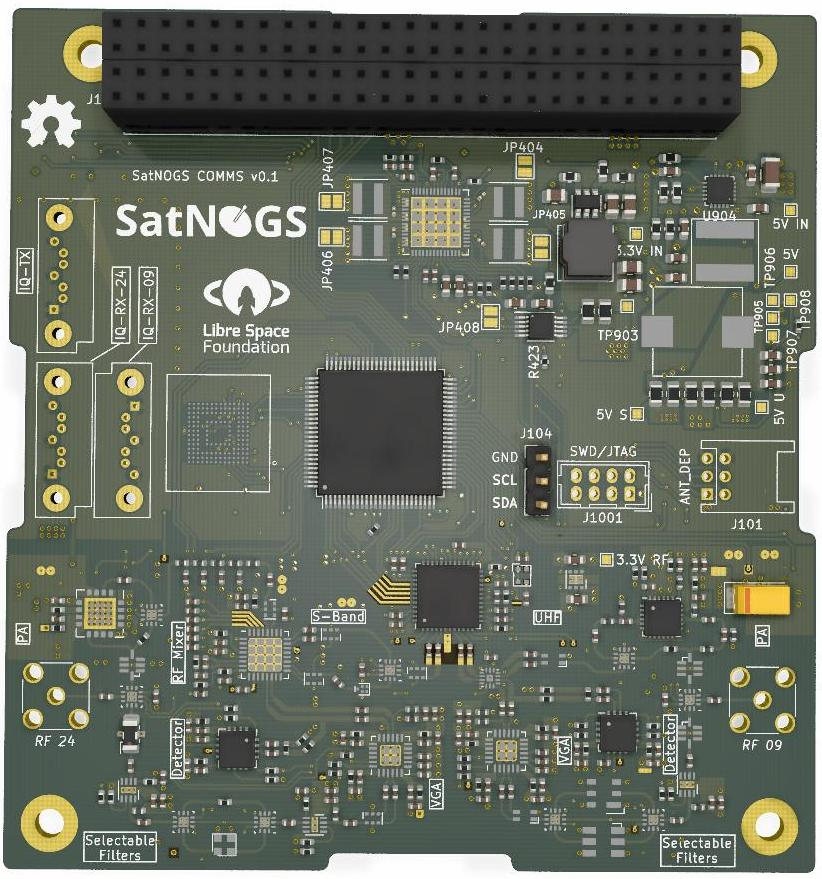
\includegraphics{satnogs-comms}
	\caption{The SatNOGS COMMS board}
\end{marginfigure}

The main component of the \acs{COMMS} subsystem is the \textbf{SatNOGS COMMS board} \autocite{surligas_satnogscomms_2021}, an open-source \acs{RF} transceiver developed by the \href{https://libre.space/}{LibreSpace Foundation}, based on \acs{CCSDS} telecommunications standards.

Communication will take place using 2 frequency bands on the \acs{ISM} range, namely \SI{436.5}{\mega\hertz} and \SI{2.425}{\giga\hertz}, supported by a deployable turnstile and a directional patch antenna respectively. The use of \acs{ISM} frequencies allows easy radio-amateur access to the satellite. The first (\acs{UHF}) band also emits a periodic \textbf{beacon}, listing information about satellite status.

The communications subsystem is also responsible for the \ac{EMC} analysis and interference mitigation, as well as the design and construction of the satellite \acl{GS}. The \acl{GS} will be part of \textbf{SatNOGS}\autocite{white_overview_satellite_2018}, a global network of satellite ground stations based on open technologies and open data.

\subsection{\acf{EPS}}
The \ac{EPS} is the subsystem responsible for the generation, distribution and storage of electrical power of the spacecraft. It is a critical aspect of the spacecraft due to the direct dependence of all subsystems to the high power needs of many CubeSat subsystems, and is theorised to be the most common reason for CubeSat failure.\autocite{langer_reliability_cubesats_2016}

AcubeSAT has opted for a \ac{COTS} subsystem approach for the \ac{EPS}:\autocite{DDJF_SYS}
\begin{itemize}
	\item \textbf{Solar panels} are procured from EnduroSat. Four 3U panels cover the \(X\) and \(Y\) faces of the satellite, and one 1U panel covers the \(-Z\) face.
	\item The \textbf{\ac{PCDU}} is procured from NanoAvionics and offers 10 switched channels with overcurrent protection over 4 voltage rails, as well as 4 \ac{MPPT} converters.
	\item The \textbf{battery pack}, also procured from NanoAvionics, contains 4 18650 Li-Ion cells in a 2S2P\footnote{2 series, 2 parallel} configuration.
\end{itemize}

\begin{margintable}
	\caption{AcubeSAT nominal mode power budget}
	\label{tab:power_budget}
	\begin{tabularx}{\linewidth}{@{}lX@{}}
		\toprule
		\textbf{Consumer}            & \textbf{Power}            \\ \midrule
		\acs{ADCS}          & \SI{1.10}{\watt} \\
		\acs{COMMS}         & \SI{0.85}{\watt} \\
		\acs{EPS}           & \SI{0.99}{\watt} \\
		\acs{OBC}           & \SI{0.12}{\watt} \\
		\acs{SU}            & \SI{0.25}{\watt} \\ \midrule
		Total               & \SI{3.30}{\watt} \\
		Orbit Average Power & \SI{4.24}{\watt} \\ \bottomrule
	\end{tabularx}
\end{margintable}

\FloatBarrier
A dynamic approach is taken with regards to power budget calculation:
\begin{compactenum}
	\item The in-orbit power generation is calculated for the duration of the mission using the \textbf{STK} software, taking into account satellite orientation, pointing profiles and eclipse, with a \SI{1}{\minute} resolution.
	\item The power consumption of the system is calculated on average for each different operational mode.
	\item \acs{MPPT} efficiencies and battery charge level are calculated for each timepoint, assuming worst-case thermal and electrical conditions
	\item A system-wide 10\% margin is applied to the results
\end{compactenum}

We have created a Python library consolidating the above steps\footurl{https://gitlab.com/acubesat/eps/power-budget} and producing the necessary outputs to prove the adequacy of the design.

\begin{figure*}[h]
%	\begin{subfigure}[b]{.45\textwidth}
	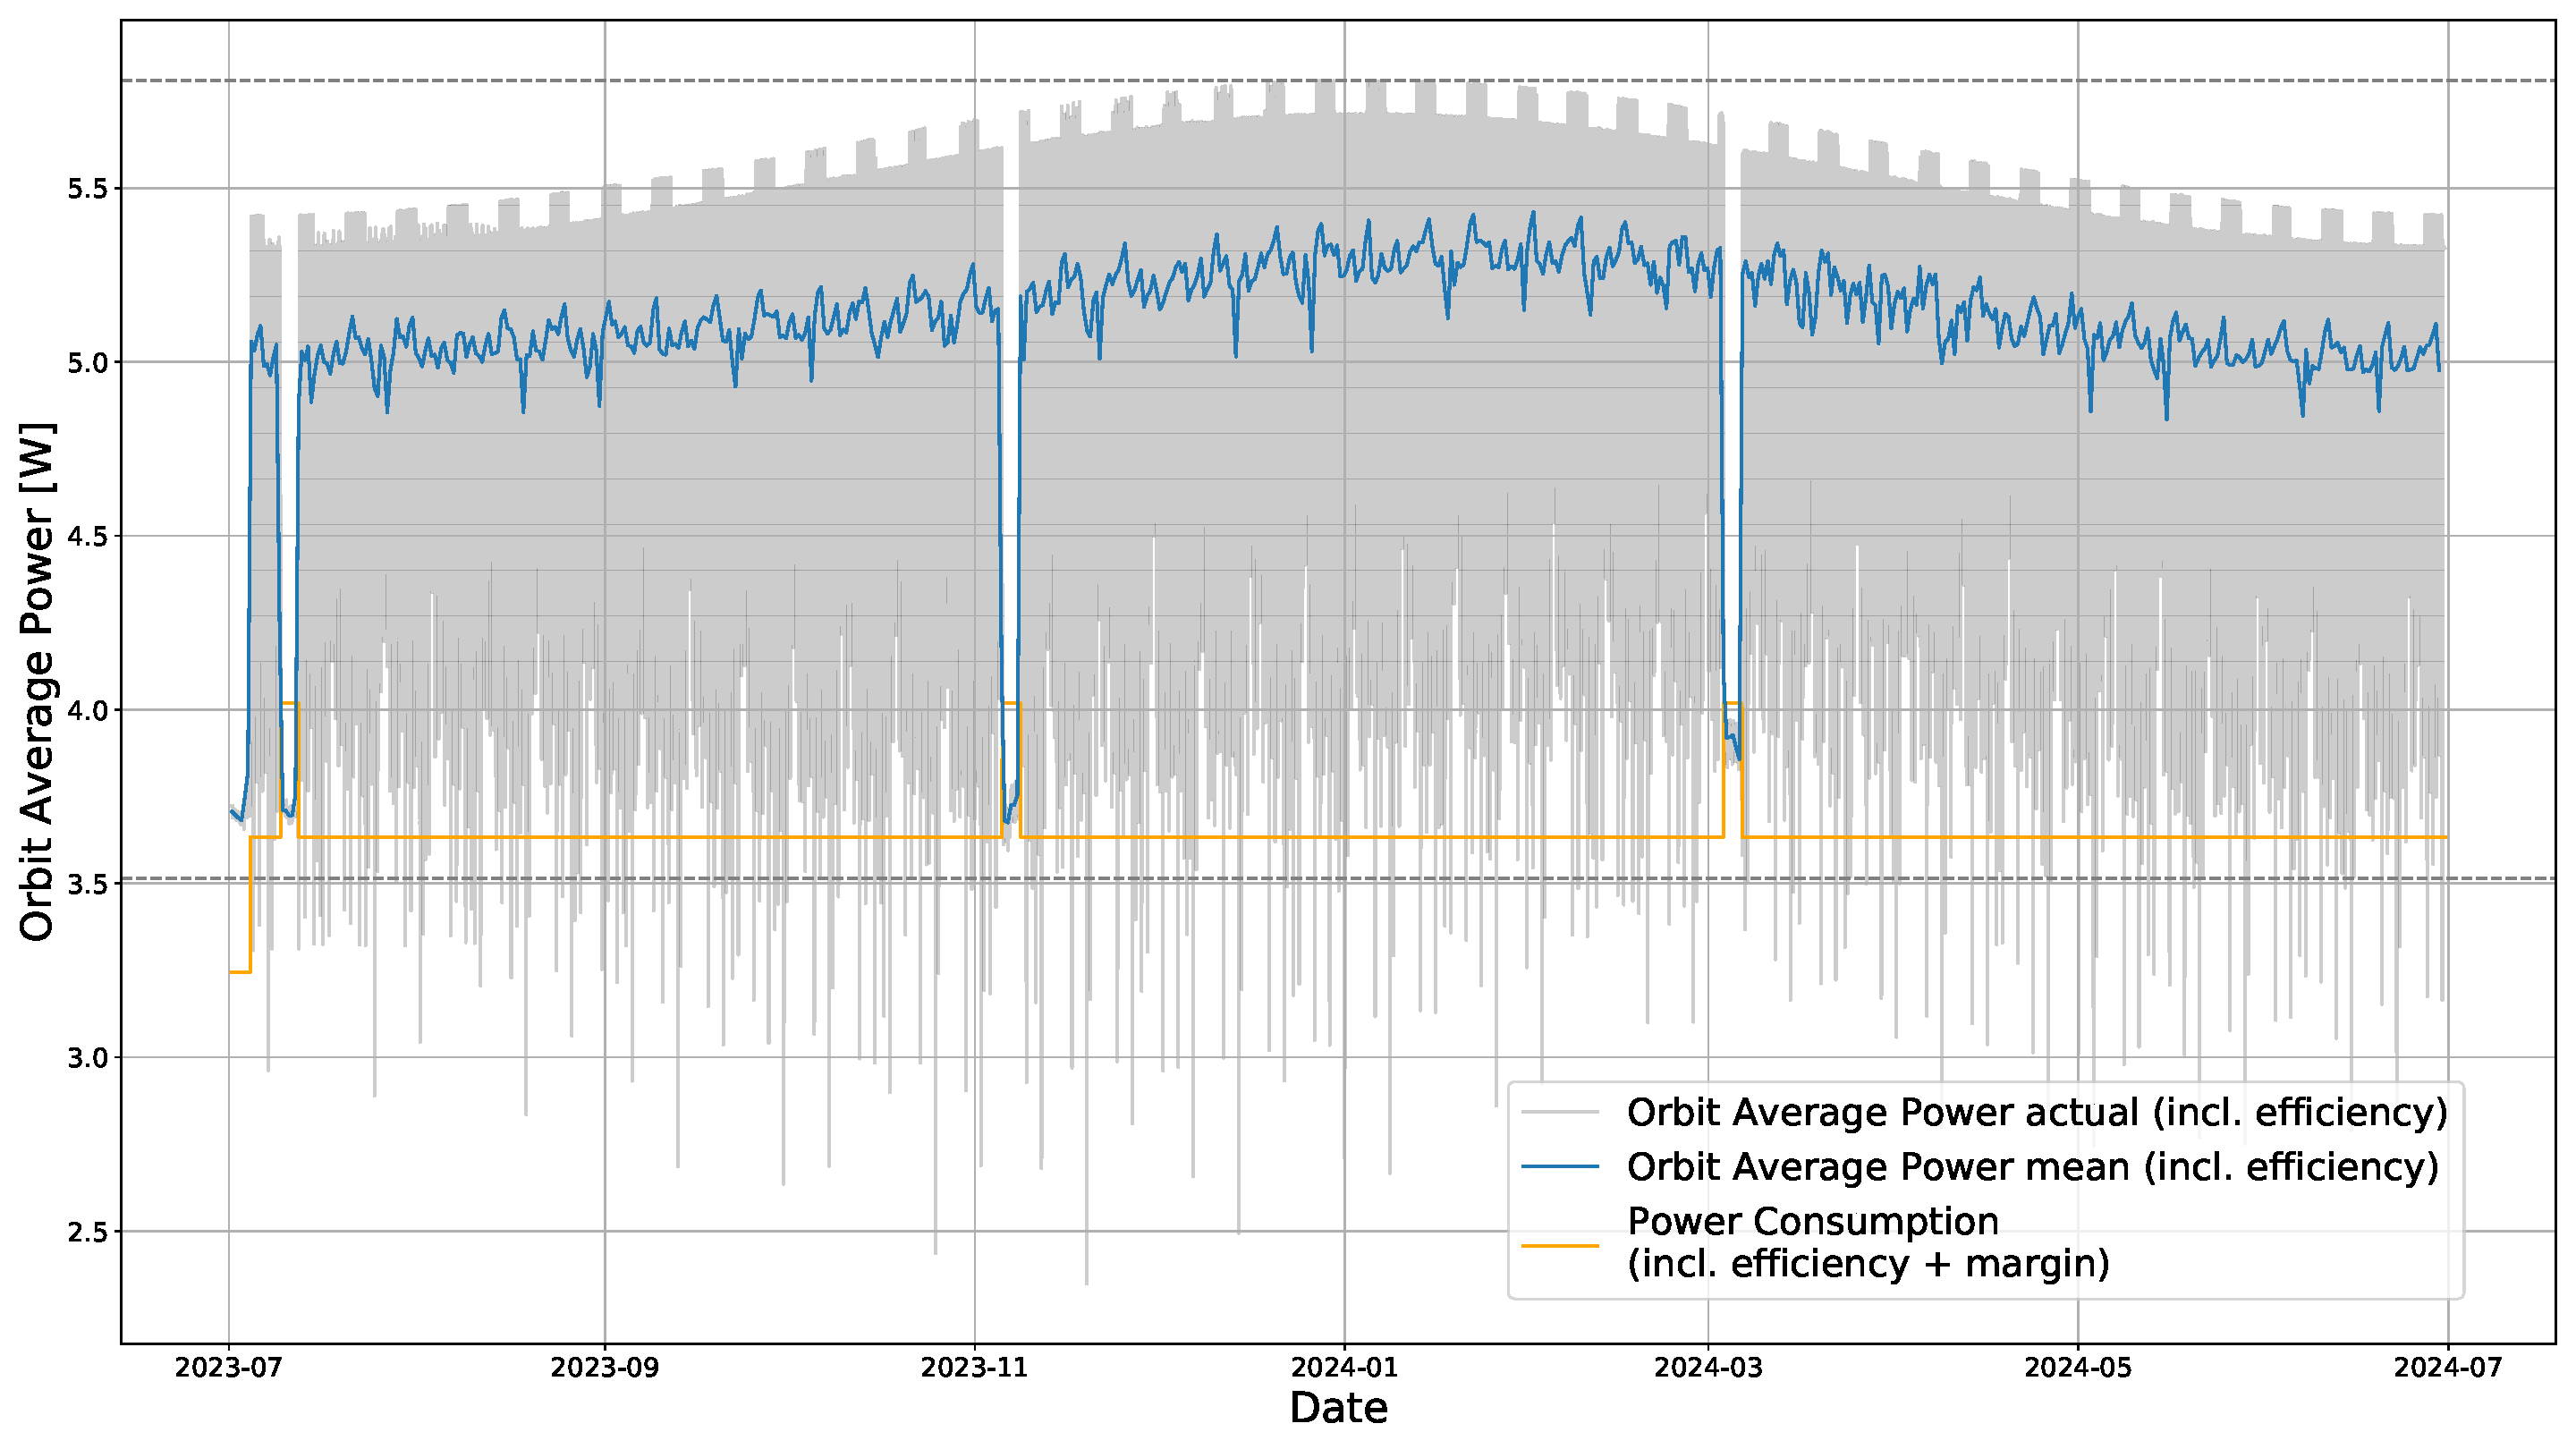
\includegraphics[height=4cm]{Sun Pointing 11:00.total.pdf}
%	\end{subfigure}
	\hfill
%	\begin{subfigure}[b]{.45\textwidth}
	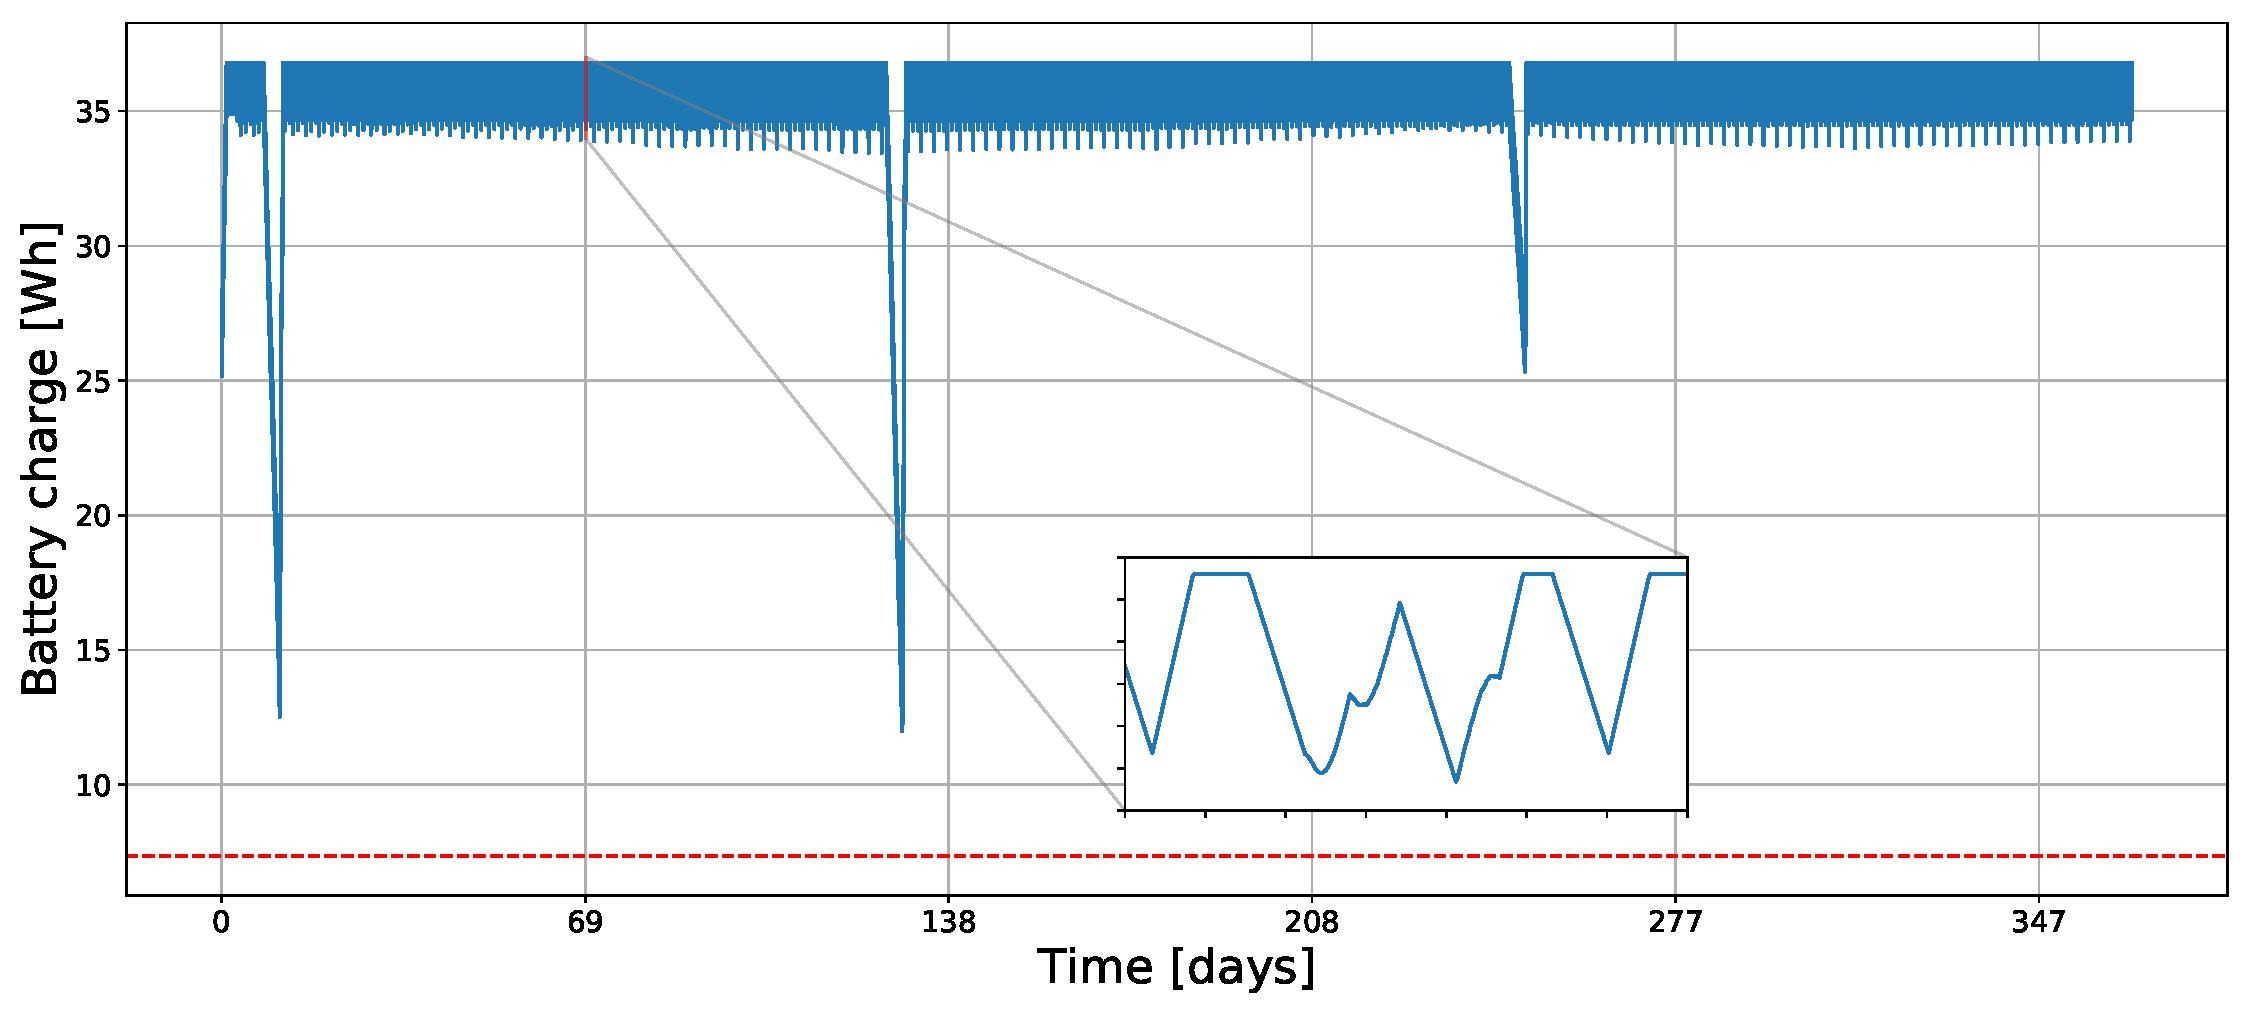
\includegraphics[height=4cm]{Sun Pointing 11:00.discharge.pdf}
%	\end{subfigure}
%	\includegraphics[width=.45\textwidth]{/home/kongr45gpen/Pictures/jeka8ara kapoglis.png}

	\caption[Dynamic power budget analysis]{Dynamic power budget analysis. Left: Power consumption \& generation for the orbit. Right: Battery discharge level throughout the mission}
\end{figure*}

\subsection{\acf{OBDH}}
\label{sec:obdh}

The \ac{OBDH} subsystem is responsible for the design of the spacecraft's data interfaces, as well as the design of the \textbf{\acf{OBC}} board, tasked with controlling the basic spacecraft functions.\autocite{DDJF_OBDH}

The \ac{OBC} board contains the main \ac{OBC} logic, and is based around a \foothref{https://www.microchip.com/wwwproducts/en/SAMV71Q21RT}{Microchip SAMV71Q21RT} radiation-tolerant microcontroller and an \acs{MRAM} memory, used to store critical data. The board also hosts the in-house implemented components of the \ac{ADCS} subsystem, as a space-saving measure.

\begin{marginfigure}
	\centering
	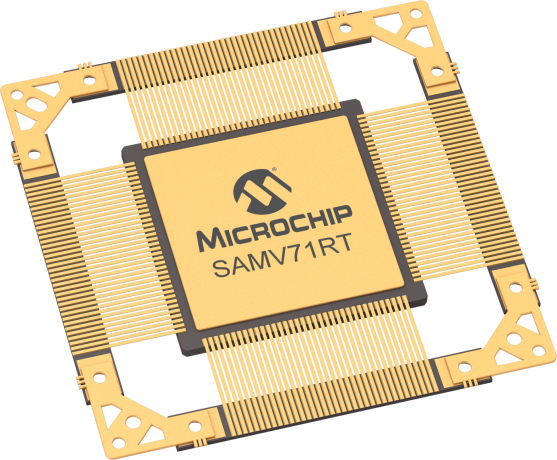
\includegraphics[width=.7\textwidth]{SAMV71Q21RT}
	\caption{The \texttt{SAMV71Q21RT} microcontroller}
	\label{fig:samv71}
\end{marginfigure}

AcubeSAT's data interface is using a cold-redundant \ac{CAN} bus to facilitate cross-subsystem communication, selected due to its robustness and reliability. \autocite{bouwmeester_survey_implementation_2017} AcubeSAT boards implement the PC/104 mechanical interface.\autocite{PC104}

\subsection{\acf{OBSW}}

The \ac{OBSW} subsystem is responsible for the design and development of the nanosatellite's software. The language chosen to be used in the system's 4 \acp{MCU} is a reduced form of \textbf{C++}, and the code is guarded under a number of standards, static checkers and unit tests.\autocite{DDJF_OBSW} All software runs under the Free\acs{RTOS} operating system.



\subsection{\acf{OPS}}

The operations subsystem is responsible for the devising the operational modes \& procedures of the spacecraft, and ensuring the functionality, commandability and observability of the satellite before and during its mission.

During flight, AcubeSAT can remain within one of the following \textbf{system modes}:\autocite{MDO}
\begin{itemize}
	\item \textbf{Launch/Off mode}: During this mode, the satellite is turned completely off, and no subsystems are energised. This is used to represent the state of the spacecraft inside the deployer, where no electronics are allowed to be energised,\autocite[req. 3.3.3]{CDS13} and the CubeSat is in a completely dormant state.
	
	\item \textbf{Commissioning mode}: This mode is initiated as soon as the CubeSat exits the deployer, meaning that launch is complete. It contains the initial startup actions of the spacecraft, including detumbling and antenna deployment. No science takes place during commissioning mode.
	
	\item \textbf{Nominal mode}: This mode represents the state where the CubeSat will spend most of the time on. Apart from the necessary autonomy functions and battery charging, the CubeSat will also downlink telemetry and science data. No science takes place during nominal mode, except for health checks commanded from the ground. Nominal mode is also the only mode where the satellite performs nadir or sun pointing (\Cref{sec:adcs}).
	
	\item \textbf{Science mode}: This is where the main experiment takes place and payload data are generated. This mode includes operation of the fluidic system, control of the microfluidic chip, reinvigoration of the cells, and periodic acquisition of pictures using the miniaturised microscope.
	
	AcubeSAT has split science mode into \textbf{3 distinct occurrences}, termed sub-experiments \(\alpha\), \(\beta\) and \(\gamma\), lasting 72 hours each, and taking place at different points of the mission to investigate the time-dependence of the observed results.
	
	\item \textbf{Safe mode}: It is common for spacecraft systems to include a \emph{safe mode},\autocite[385]{aguirre_introduction_space_2013} where the spacecraft switches off all non-essential systems and function, in order to respond to major malfunctions that cannot be corrected by autonomous procedures. Safe mode is intended as a well-defined and well-tested mode which is easy to maintain and reduces risk of any malfunction.
	
	On AcubeSAT, spacecraft functionality is significantly reduced, and the attitude profile includes pointing only. However, \ac{UHF} communication and beacon transmission are still active for observability purposes.
\end{itemize}

\begin{table*}[h]
	\centering
	\caption{Overview of AcubeSAT functionality on different modes}
	\label{tab:acubesatmodes}
	\begin{tabular}{@{}llllll@{}}
		\toprule
		Function    & Launch & Commissioning  & Nominal                 & Science        & Safe             \\ \midrule
		\acs{ADCS}  & \color{off} Off    & Detumbling     & \color{on} Pointing                & Detumbling     & Detumbling       \\
		\acs{COMMS} & \color{off} Off    & \acs{UHF} only & \color{on} \acs{UHF} and S-Band    & \acs{UHF} only & \acs{UHF} only   \\
		\acs{EPS}   & \color{off} Off    & \color{on} On             & \color{on} On                      & \color{on} On             & \color{on} On               \\
		\acs{OBC}   & \color{off} Off    & \color{on} On             & \color{on} On                      & \color{on} On             & \color{on} On               \\
		\acs{SU}    & \color{off} Off    & \color{off} Off            & Maintenance \& data only & \color{on} On             & Maintenance only \\ \bottomrule
	\end{tabular}
	\vspace{1em}
\end{table*}


Each mode is associated with a \textbf{functional flow} diagram, showing a high-level description of the spacecraft operation during this mode.\autocite{acubesat_functional_2021}

\begin{figure}
	\centering
	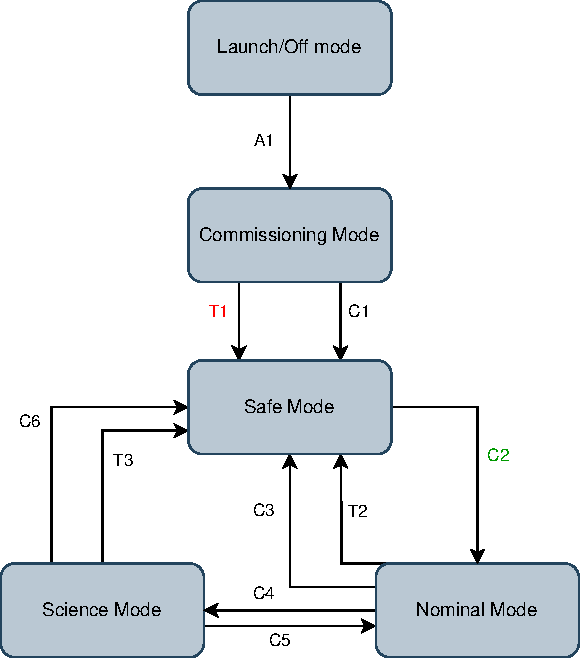
\includegraphics[width=.6\textwidth]{AcubeSAT_System_Modes}
	\caption[][3cm]{All transitions between system modes}
	\label{fig:transitions}
\end{figure}


\subsection{Structural}

The Structural subsystem has taken over:
\begin{itemize}
	\item The analysis and configuration of the \ac{COTS} 3-unit structure (\Cref{fig:structure}) housing all the CubeSat's components. Vibration analyses are especially important, as they serve to investigate whether the CubeSat can withstand the launcher's loads.
	\item The complete design, manufacturing and assembly of the \textbf{payload container} and its unibody, hosting the scientific experiment of the mission (\Cref{fig:container}).
\end{itemize}

\begin{marginfigure}
	\centering
	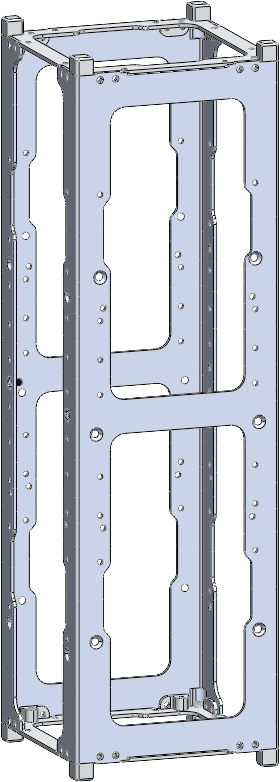
\includegraphics[width=.5\textwidth]{structure}
	\caption{The CubeSat's 3U \acs{COTS} structure}
	\label{fig:structure}
\end{marginfigure}

\subsection{\acf{SYE}}

The \acl{SYE} subteam serves as the technical authority for the satellite. It is responsible for coordinating the developments and interfaces between subsystems, ensuring the conformance to standards and technical requirements, and identifying \& resolving all issues arising from the complex multi-discipline design of the CubeSat.

Additionally, the \ac{SYE} team is responsible for some specific technical developments that do not belong in any of the other subsystems, such as \ac{RAMS}, \ac{FMEA}, harnessing and the \acl{MAIV} plan.

\subsection{\acf{SU}}

The \acl{SU} subteam is responsible for the conceptualisation and implementation of the mission's scientific payload, namely the high-throughput study of the effects of \ac{LEO} environments on yeast cells.

The payload is composed of the following functional parts:\autocite{DDJF_PL}
\begin{compactitem}
	\item The \textbf{payload container}, an almost 2U aluminum structure, pressurised at standard atmospheric pressure, and designed to host all the payload instrumentation. The container also accomodates a unibody which mechanically supports all \ac{SU} components.
	\item A \textbf{microfluidic chip} based on \ac{PDMS}, hosting 384 chambers capable of probing 190 distinct strains of \emph{Saccharomyces Cerevisiae} for each subexperiment.
	\item A \textbf{fluidic system} composed from 2 pumps, 8 latching solenoid valves, 6 non-latching solenoid valves, and 3 fluid medium containers
	\begin{marginfigure}
		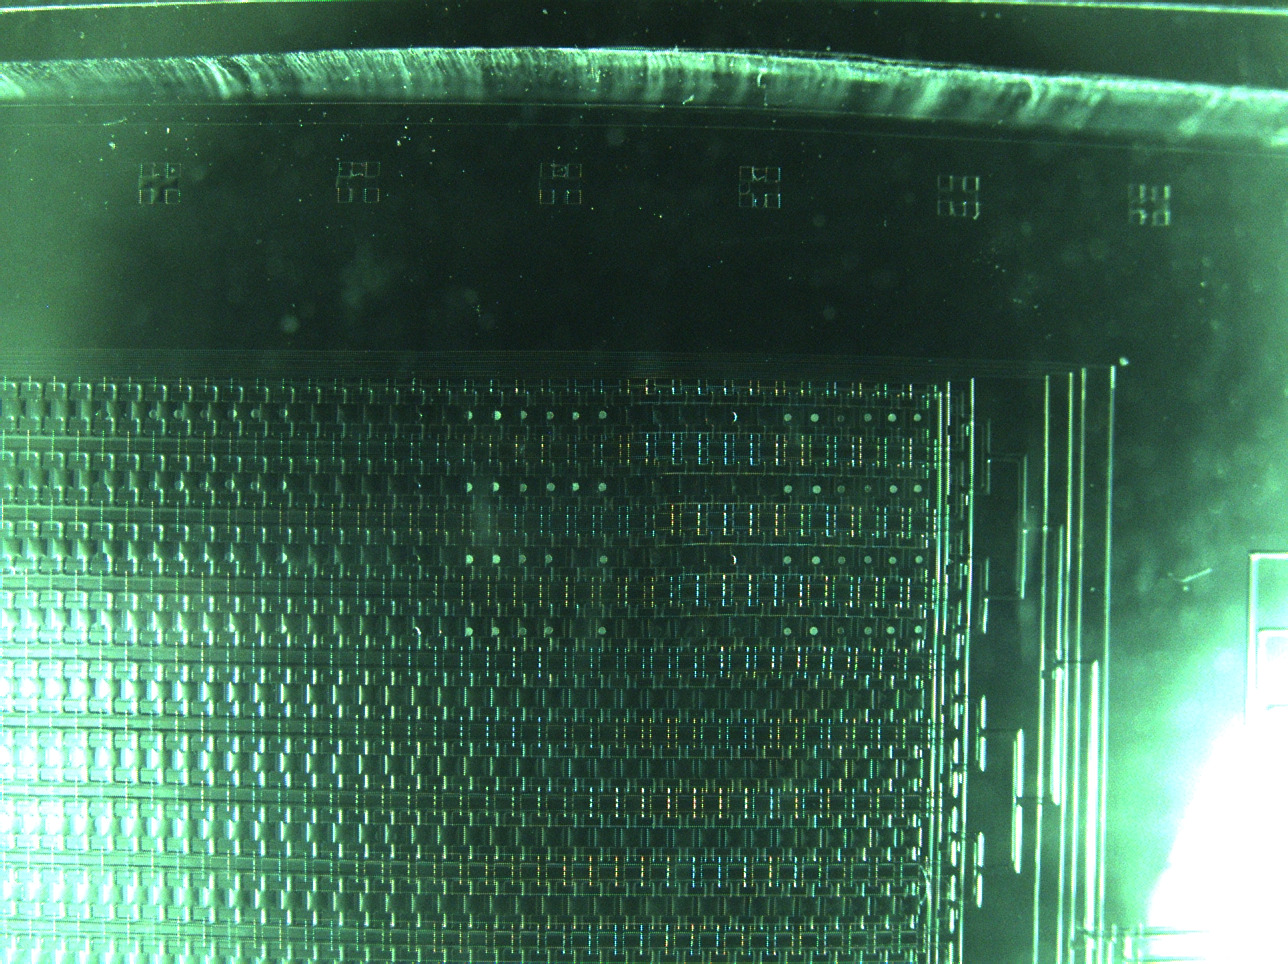
\includegraphics{chipFluor}
		\caption[Example mission image output]{Example mission image output (\parencite{DDJF_PL})}
		\label{fig:chip_fluor}
	\end{marginfigure}
	\item An \textbf{imaging system} operating as a microscope, containing a camera and a series of lights, filters and a lens
	\item A number of \textbf{heaters} to control component operational temperatures
	\item A number of redundant \textbf{sensors} for environmental measurements
	\item A \ac{PCB} containing the microcontroller and rest of the control components of the payload
\end{compactitem}

\begin{marginfigure}
	\centering
	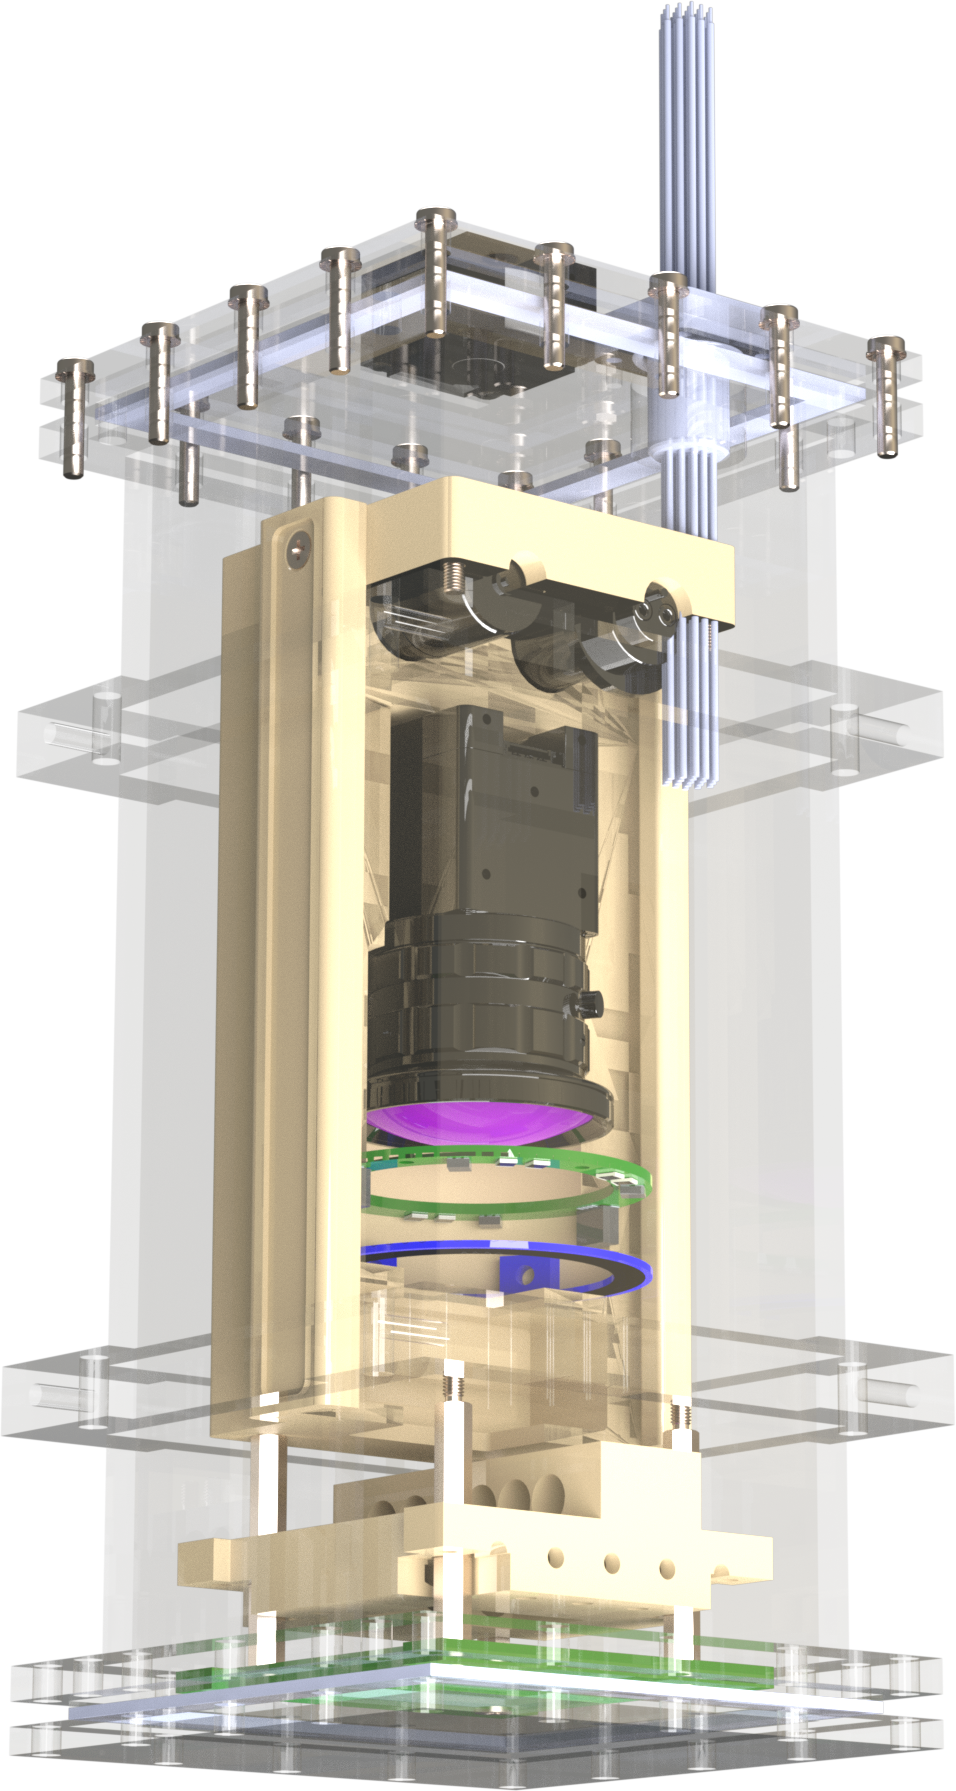
\includegraphics[width=.9\textwidth]{Glass_Payload}
	\caption{Transparent view of the payload container and its internals}
	\label{fig:container}
\end{marginfigure}

There is a number of constraints that the payload imposes on \ac{FDIR} design:
\begin{enumerate}
	\item \textbf{Interruption} of one of the three 72-hour subexperiments during execution may mean complete loss of the subexperiment. The impact of such an event depends on the duration and timepoint of its occurence. In any case, adequate observability will allow the ground-control experiment to mimic the in-orbit conditions as much as possible.
	\item \textbf{Freezing} of liquids inside the chip and fluidic tubes may lead to permanent damage on the setup. As such, heater operation may be required even during safe mode, after the first sub-experiment has been performed and liquid has flown into the system. This characteristics imposes further restrictions on the minimum availability of the system, depending on the thermal conditions.
\end{enumerate}

\begin{figure*}
	\centering
	\caption[The microfluidic chip and its separation into 3 subexperiments and 1 test line]{The microfluidic chip and its separation into 3 subexperiments and 1 test line. The fluid inlets are shown on the left side of the chip, while the outlets are on the right. \emph{Green:} flow layer. \emph{Blue:} control layer.}
	\label{fig:chip}
	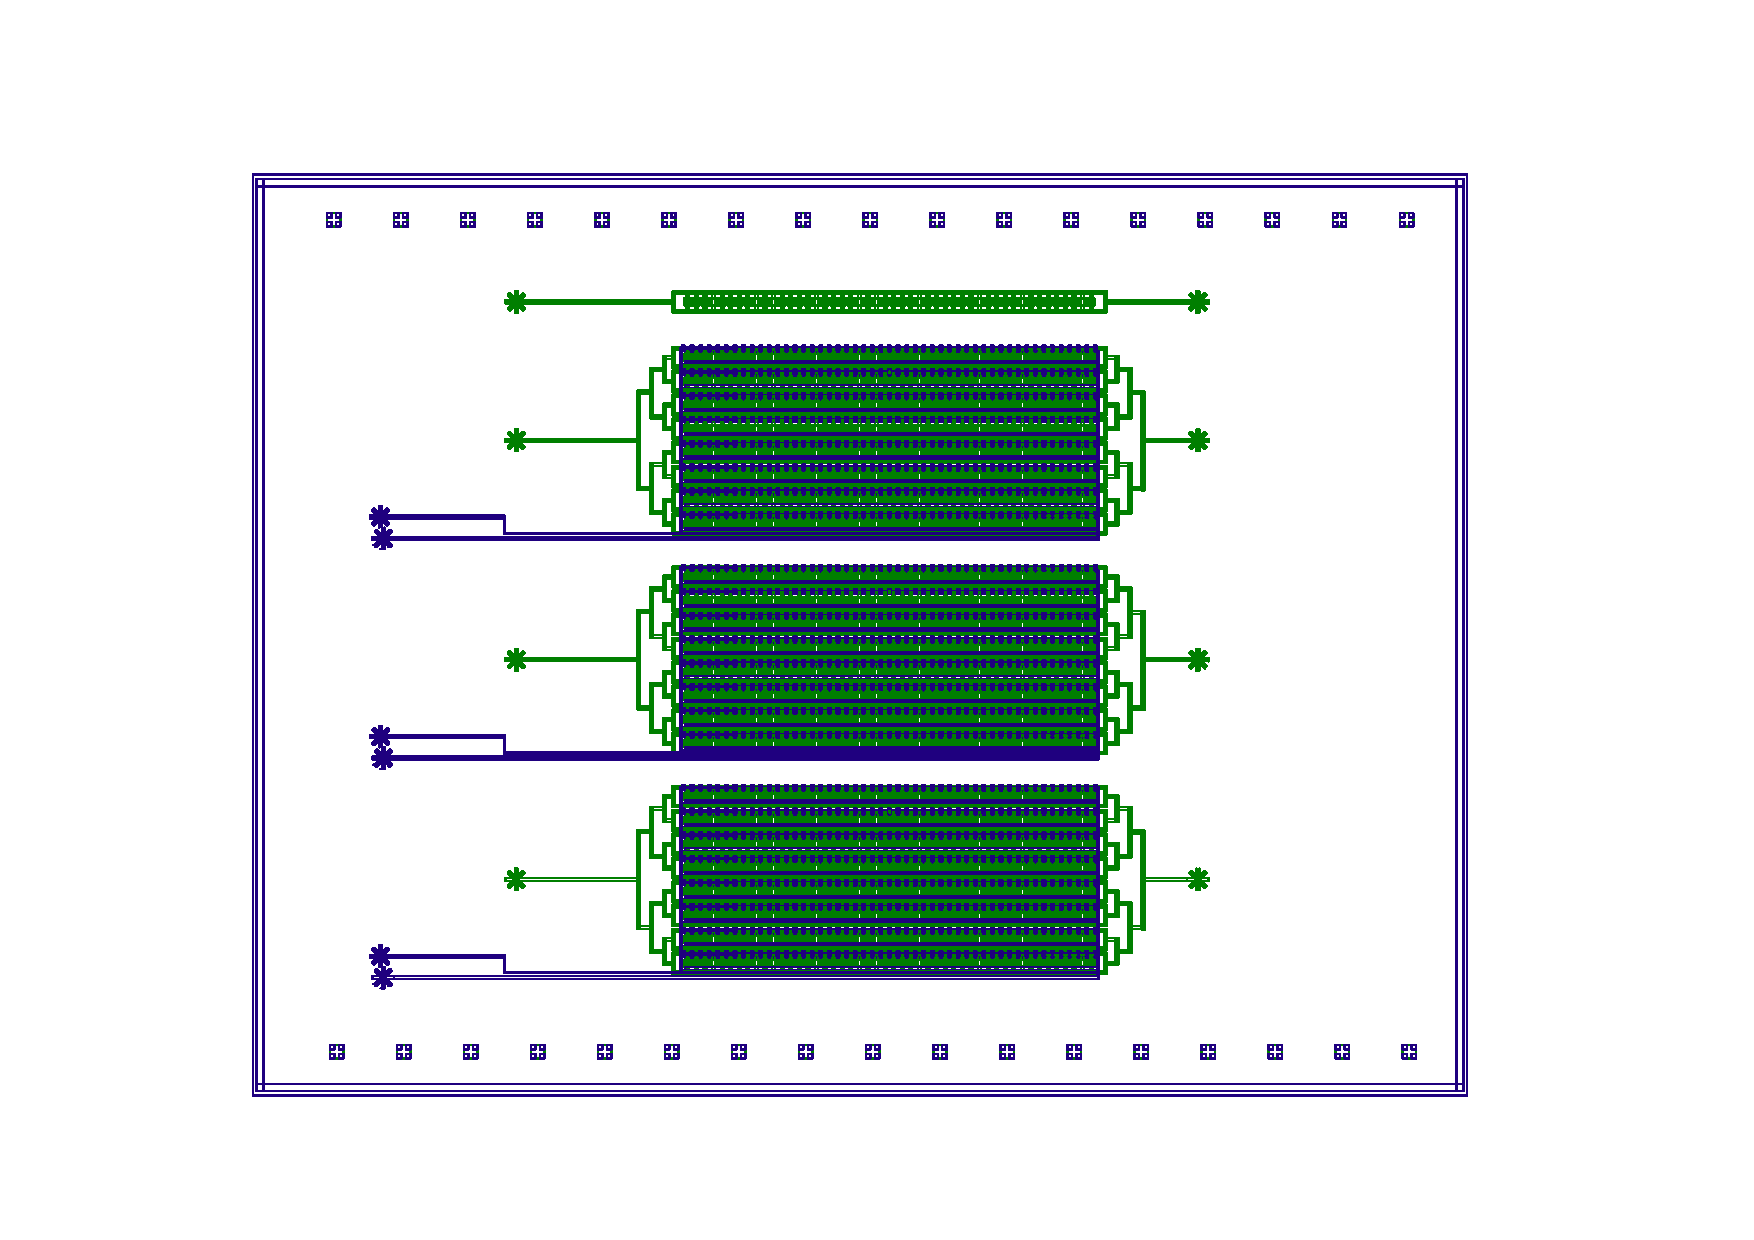
\includegraphics{final_chip.pdf}
	\begin{tikzpicture}[overlay]
	\draw[very thick,dashed,solarized-base01] (5,10.9) rectangle (-7,11.5) node[below right] {Test line};
	\draw[very thick,dashed,solarized-green] (5,7.85) rectangle (-7,10.8) node[below right] {Subexperiment $\alpha$};
	\draw[very thick,dashed,solarized-blue] (5,4.95) rectangle (-7,7.8) node[below right] {Subexperiment $\beta$};
	\draw[very thick,dashed,solarized-red] (5,2) rectangle (-7,4.9) node[below right] {Subexperiment $\gamma$};
	\end{tikzpicture}
\end{figure*}

\subsection{Thermal}

The Thermal subteam is responsible for the thermal analysis of the satellite, where the solar and earth albedo conditions are combined with the components' heat dissipation to determine the worst-case temperatures experienced by the satellite in hot and cold conditions.

The results of thermal analysis typically lead to implementation of passive or active thermal control methods. Notably, in AcubeSAT, 3 electronically-controlled heaters are used for the batteries, \acs{PDMS} chip and valves.

\subsection{Trajectory}

The Trajectory subteam is responsible for the analysis of the spacecraft's orbit, the calculation of radiation effects, the satellite's compliance to space debris regulations, and the estimation of its orbital lifetime.

AcubeSAT's requirements do not dictate use of thrusters, meaning that the satellite's orbit will be determined solely by the launcher, and cannot be altered in flight. As the selected launcher opportunity is unknown until some time before satellite delivery, a number of sensitivity analyses are executed to determine the allowed orbits.

\begin{figure}
	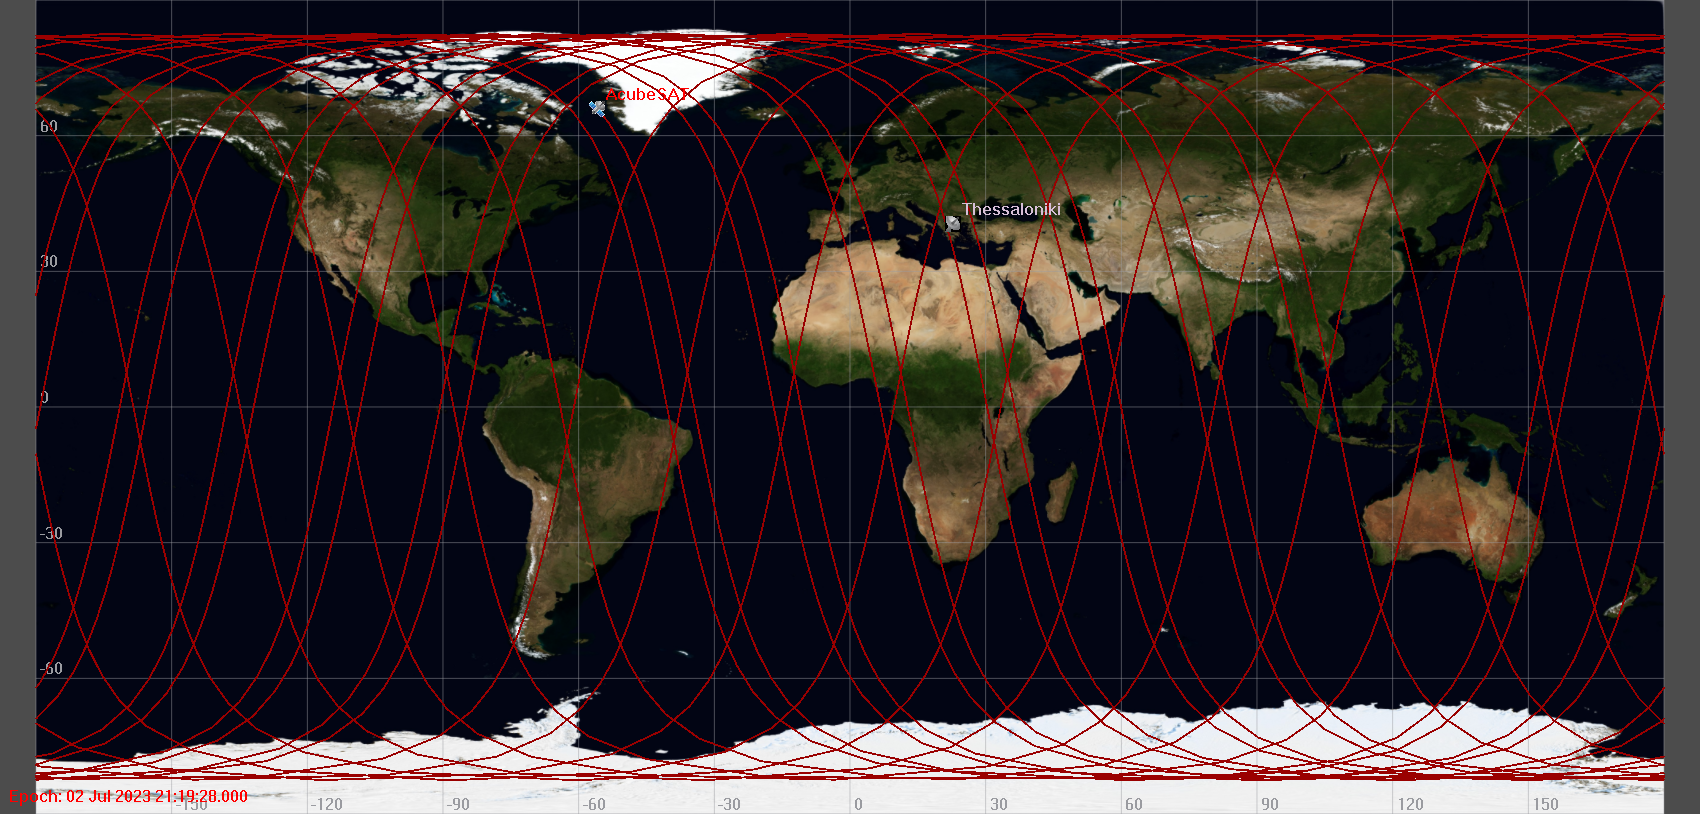
\includegraphics{GmatScreenShot_002}
	\caption[Ground track of an example AcubeSAT orbit, generated using NASA's GMAT]{Ground track of an example AcubeSAT orbit, generated using NASA's \acl{GMAT}}
	\label{fig:gmat}
\end{figure}

% Maybe add some info about the sensitivity results and LTAN value?

\section{Tools used}
\draft{Here we write a small paragraph about OCDT and other MBSE tools and utilities used by AcubeSAT or developed in-house...}

\chapter{The SAVOIR \ac{FDIR} concept}

\section{The \acs{ECSS} \acl{PUS}}

\subsection{The \acs{ECSS} services}

\begin{figure}
	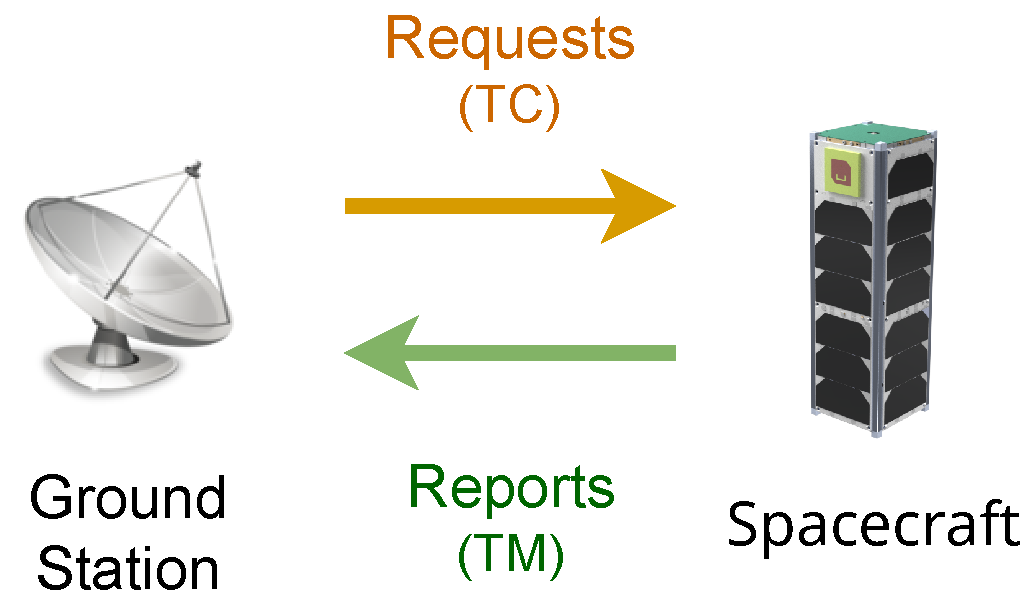
\includegraphics{ECSS-rq}
	\caption[][-1em]{The \ac{PUS} data transfer model}
	\label{fig:pusmodel}
\end{figure}

blablablab \autocite{ECSS-E-ST-70-41C,ECSS-E-70-41A,kaufeler_esa_standard_1994}

\begin{compactitem}
	\item \textbf{\texttt{ST[01]}: Request verification}
	
	Provides acknowledgement or failure reports for executed commands. This service essentially informs the operators about the status of \ac{TC} sent to the spacecraft, and reports any occurred errors during parsing or execution.
	
	\item \textbf{\texttt{ST[02]}: Device access}
	
	Allows toggling, controlling and reconfiguring any on-board peripherals that do not support the \ac{PUS} paradigm, but rely on simpler protocols to communicate.
	
	\item \textbf{\texttt{ST[03]}: Housekeeping}
	
	Produces periodic reports containing values of on-board parameters. This service essentially composes the periodic \acs{RF} \textbf{beacon} of the satellite, by storing and transmitting parameter values without any prior \acs{TC} request.
	
	\item \textbf{\texttt{ST[04]}: Parameter statistics reporting}
	
	Allows reporting statistics (min, max, mean, standard deviation) for specific parameters over specified intervals. This is a memory-efficient alternative to the \texttt{ST[03]} housekeeping service.
	
	\item \textbf{\texttt{ST[05]}: Event reporting}
	
	Generates reports when notable occurrences take place on-board, such as:
	\begin{compactitem}
		\item Autonomous on-board actions
		\item Detected failures or anomalies
		\item Predefined steps during an operation
	\end{compactitem}
	
	\item \textbf{\texttt{ST[06]}: Memory management}
	
	Allows writing and reading directly from an on-board memory unit. This can be useful for debugging and investigative purposes, fetching mission data, or uploading new software to the spacecraft avionics. The service also provides for downlinking and uplinking files in a file system.
	
	\item \textbf{\texttt{ST[07]}: Task management} \emph{(deprecated)}
	
	Allows stopping, suspending or resuming software tasks in case of contingency. This service has been removed from the standard and is only mentioned as a reference.
	
	\item \textbf{\texttt{ST[08]}: Function management}
	
	Provides the capability of running predefined actions that can receive further parameters. These actions can correspond to payload, platform, or any other functionality.
	
	\item \textbf{\texttt{ST[09]}: Time management}
	
	Allows periodic reporting of the current absolute spacecraft time for observability and correlation purposes.
	
	\item \textbf{\texttt{ST[10]}: Time packet} \emph{(deprecated)}
	
	Used in the past for time packet generation. This service has been removed from the standard and is only mentioned as a reference.
	
	\item \textbf{\texttt{ST[11]}: Time-based scheduling}
	
	Allows the operators to \textbf{"time-tag"} telecommands for execution at future timestamps, instead of immediately.
	
	\item \textbf{\texttt{ST[12]}: On-board monitoring}
	
	This service allows checking parameter values to ensure that they remain within configurable limits. Whenever a violation occurs, an \texttt{ST[05]} can be optionally generated for further processing.
	
	\item \textbf{\texttt{ST[13]}: Large packet transfer}
	
	Provides a method of message segmentation, for message payloads that are too large to fit within the maximum allowed length for \ac{TC} or \ac{TM}.
	
	\item \textbf{\texttt{ST[14]}: Real-time forwarding control}
	
	This service is responsible of controlling which types of generated reports are immediately transmitted to the \acl{GS}.
	
	\item \textbf{\texttt{ST[15]}: On-board storage and retrieval}
	
	This service allows storing generated report on-board, as well as their commanded mass retrieval when the spacecraft has \acl{GS} visibility.
	
	\item \textbf{\texttt{ST[16]}: On-board traffic management} \emph{(deprecated)}
	
	Allows monitoring the status and load of an on-board data bus and provides commands for resolution of errors. This service has been removed from the standard and is only mentioned as a reference.
	
	\item \textbf{\texttt{ST[17]}: Test}
	
	This service allows performing on-board connection and "are-you-alive" checks.
	
	\item \textbf{\texttt{ST[18]}: On-board operations procedure}
	
	Allows loading, controlling (start, suspend, resume, abort) and configuring On-Board Control Procedures, which are sequences of commands written in an application-specific language.
	
	\item \textbf{\texttt{ST[19]}: Event-action}
	
	Provides the operators with the capability of autonomously executing \acp{TC} when an \texttt{ST[05]} event is triggered.
	
	\item \textbf{\texttt{ST[20]}: On-board parameter management}
	
	Provides the capability of reading and setting on-board parameters. Parameters are some of the most important entities defined in the \acs{PUS}, and can represent:
	\begin{itemize}
		\item Read-write configuration variables for the system or lower-level components
		\item Read-only sensor and other telemetry values
		\item \ac{FDIR} results and diagnostics
	\end{itemize}
	
	\item \textbf{\texttt{ST[21]}: Request sequencing}
	
	Allows operators to load series of \acp{TC} to be executed in a sequential order.
	
	\item \textbf{\texttt{ST[22]}: Position-based scheduling}
	
	Provides the capability of executing \acp{TC} when the spacecraft reaches a specific point in its orbit.
	
	\item \textbf{\texttt{ST[23]}: File management}
	
	Provides the capability of managing on-board file systems, with functions such as \emph{copy}, \emph{move}, \emph{delete}, or \emph{create directory}.
\end{compactitem}

\section{The SAVOIR standard}

\begin{figure*}[h]
	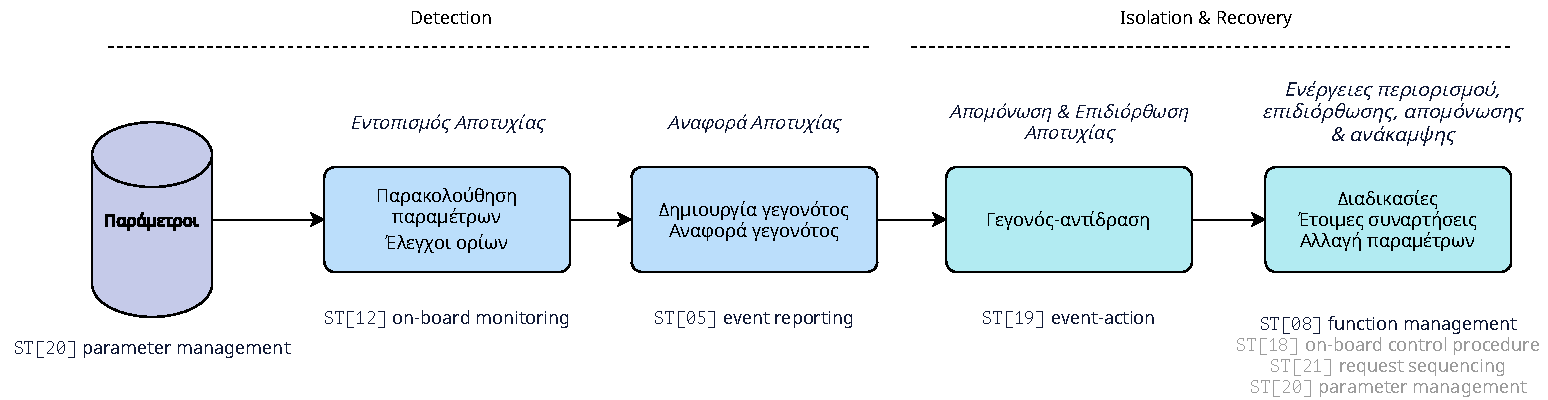
\includegraphics{../cdr/04 FMEA/media/FDIRpus}
	\caption{blablabla}
\end{figure*}

\chapter{\ac{FDIR} in AcubeSAT}

\section{\ac{FDIR} principles}

\draft{\begin{itemize}
		\item The 7 AcubeSAT FDIR principles
		\item SAVOIR FDIR requirements and compliance
\end{itemize}}

\section{Investigation on different architectures}

\begin{figure}
	\centering
	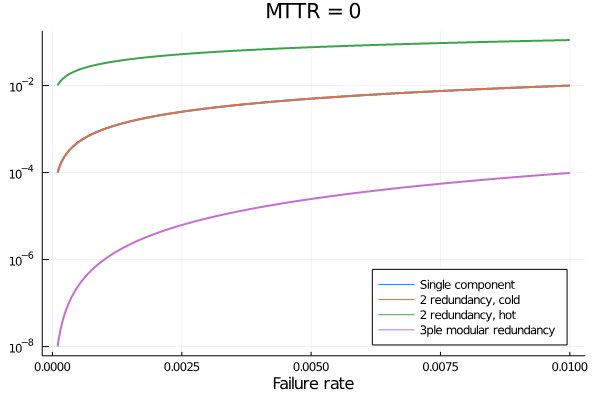
\includegraphics[width=.5\textwidth]{demoplot}
	\caption{\draft{Error rates}}
\end{figure}

\FloatBarrier
\section{Failure causes and recovery actions}

\subsection{Failure causes}

\subsection{Preventive actions}

\subsection{Corrective actions}

\section{\ac{FDIR} operating modes}
\label{sec:fdir_operating_modes}

\chapter{Practical demonstration of \ac{FDIR}}

As a proof of concept for AcubeSAT's \ac{FDIR} implementation, a practical setup to simulate the satellite's behaviour was prepared (\Cref{fig:block}). Key elements of the setup are:
\begin{compactitem}
	\item A Cortex-M7 \textbf{microcontroller}, used to simulate a \textbf{satellite subsystem}
	\item A number of redundant \textbf{sensors} used as the potential failure points
	\item The accompanying \textbf{software} that includes an implementation of the \ac{ECSS} services and the \ac{SAVOIR} \ac{FDIR} methodology
	\item A desktop computer, serving as the \textbf{ground station} to provide the necessary commanding and observing capabilities
\end{compactitem}

\begin{figure*}[h]
	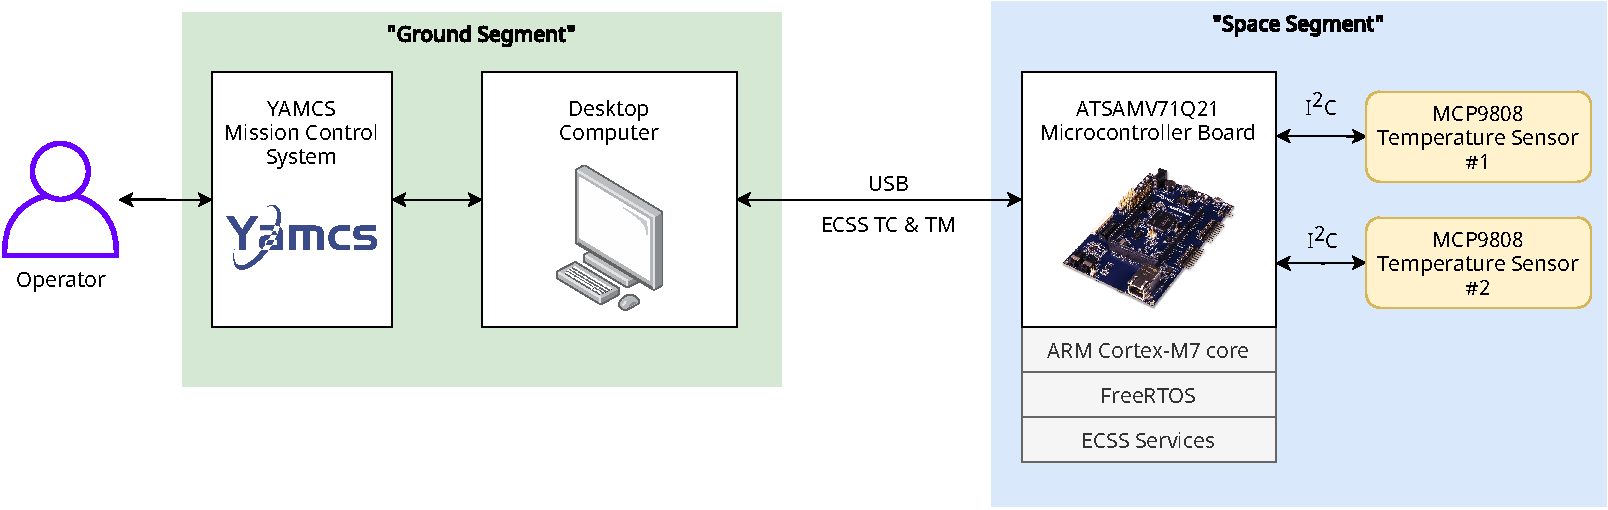
\includegraphics{SystemDescription}
	\caption{High-level block diagram of the demonstration system}
	\label{fig:block}
\end{figure*}

\section{System Description}

\subsection{Functionality}
\label{sec:tsvcd}

In order to emulate the most core functions of a spacecraft subsystem, we implemented a system with a single functional requirement:
\begin{quote}
	\texttt{RQ-010}: The system shall measure and report the ambient temperature.
\end{quote}

In order to justify implementing an \ac{FDIR} approach for this system, we will introduce a reliability requirement:
\begin{quote}
	\texttt{RQ-020}: No single failure on any measuring component shall lead to loss of system functionality
\end{quote}

The detailed design of this simple demonstration system is presented in the following sections, and was architected to match the functionality, interfaces, design and software of the AcubeSAT nanosatellite as much as possible.

\subsection{Hardware}

The centre of the demonstration system is the \ac{MCU} used to simulate the design and functionality of one of AcubeSAT's subsystems (\Cref{sec:obdh}). The selected \ac{MCU} is the Atmel \texttt{ATSAMV71Q21} hosted on the \foothref{https://www.microchip.com/Developmenttools/ProductDetails/ATSAMV71-XULT}{\texttt{ATSAMV71-XULT}} development board. This \ac{MCU} is functionally identical to the one that will be used in orbit, featuring a 32-bit ARM Cortex-M7 core with \SI{2}{\mebi\byte} of flash and \SI{384}{\kibi\byte} of \acs{SRAM} memory, and a maximum clock speed of \SI{300}{\mega\hertz}.

The \ac{MCU} is accompanied by two \textbf{temperature sensors} which are used to simulate subsystem components which are prone to failure. The selected sensor is the Microchip \foothref{https://www.microchip.com/wwwproducts/en/MCP9808}{\texttt{MCP9808}} which offers an accurate and frequent temperature readout over an \ac{I2C} bus. The maximum acquisition interval for the sensor is \SI{250}{\milli\second}.

\marginnote{%
\textbf{Cold redundancy:} Only one component is operating, while the other is not.

\textbf{Warm redundancy:} One component is operating fully, and the other is operating with reduced functionality.

\textbf{Hot redundancy:} Two or more simultaneously active parts operate in parallel. \parencite{SAVOIR-HB-003}
}

The two sensors are wired in a \textbf{hot-redundant} configuration, due to their extremely low operating power. The two sensors are connected to different \ac{I2C} buses, so that the failure of one bus will not affect the operation of the other sensor.

\paragraph{\acs{USB} interface} In order to receive \acl{TM} and transmit \acl{TC} to the demonstrative space segment, a \acs{USB} link with a desktop computer is integrated into the design. This link uses the \acs{UART} peripheral of the microcontroller, which solely transfers \acs{ECSS} messages between the microcontroller and the desktop. These messages include the typical \acs{TM} reports and \acs{TC} requests, but also log messages intended for diagnostic purposes.

As the \acs{UART} protocol does not offer packetisation facilities by default, \ac{COBS} encoding \autocite{cheshire_consistent_overhead_1997} is implemented for all transmitted messages.

\begin{figure*}[h]
	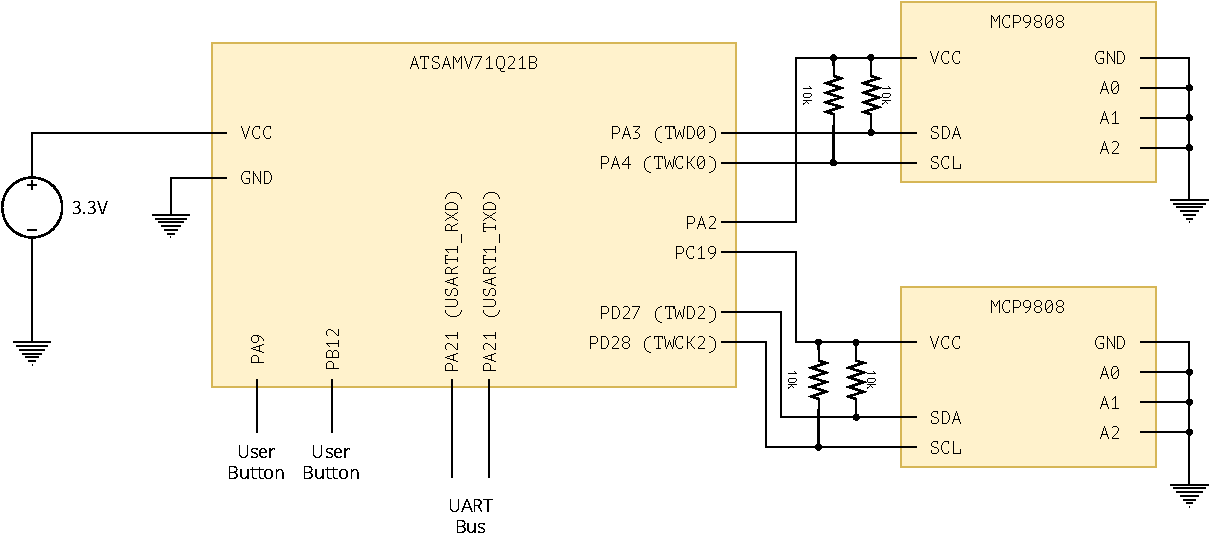
\includegraphics{ElectricalSchematic}
	\caption{Electrical schematic of the implementation}
	\label{fig:schematic}
\end{figure*}

\paragraph{Connections}
The development board and sensors were laid out and connected directly. The sensor \acp{IC} were soldered on breakout \acp{PCB} which were manufactured based on Jaroslav Sýkora's design.\url{https://www.jsykora.info/2019/06/pcb-panel-\-of-smt-breakout-boards-soic-tssop-msop/}

\section{Software}

\subsection{Flight Segment}

All \ac{FDIR} operations and functionality are developed using the \textbf{C++} language\footnote{The \texttt{C++17} standard has been selected} on the \ac{MCU}. All developments rely on free and open source software which is freely available for download and modification. The \foothref{https://git-scm.com/}{Git} version control is used for all software projects.

The \ac{FDIR} functionality is structured around the \textbf{ECSS-E-ST-70-41C \ac{PUS} implementation created by the AcubeSAT team}\footnote{\url{https://gitlab.com/acubesat/obc/ecss-services}}, which offers a modular implementation of the standard utilising modern C++.

The \ac{MCU} software and business logic are built on \textbf{\foothref{https://www.freertos.org/}{Free\acs{RTOS}}}, a low-footprint real-time operating system targeted towards embedded devices. FreeRTOS provides the capability of safe concurrency, along with support for well-controlled tasks and a number of synchronisation primitives.

\begin{figure*}[h]
	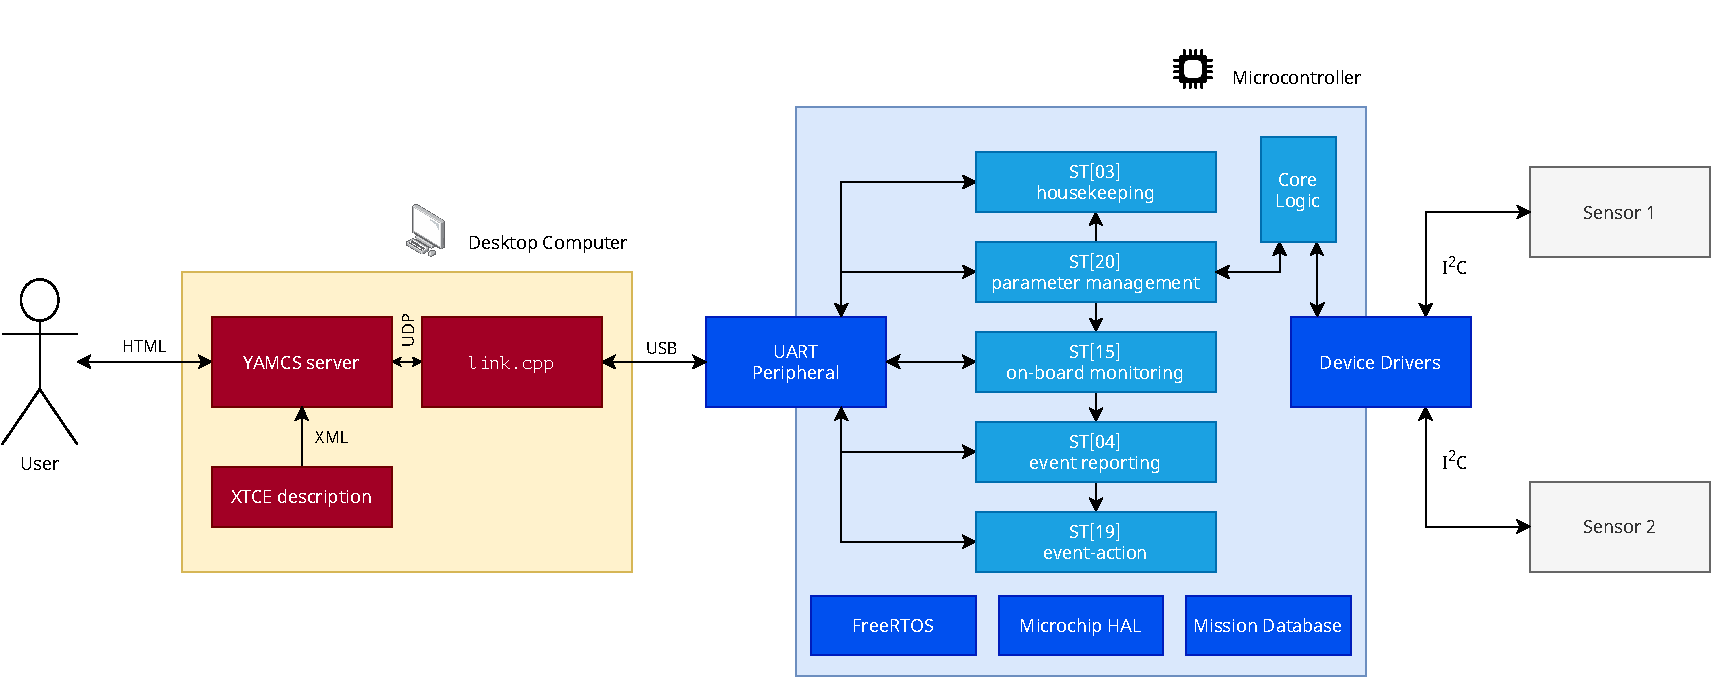
\includegraphics{SoftwareFlow}
	\caption{View of the software components and the data flow between them}
	\label{sec:softwareflow}
\end{figure*}

To ensure high reliability and a low resource footprint of the software, the following \textbf{constraints} are enacted in C++ development:
\begin{compactenum}
	\item Dynamic memory allocation\footnote{Use of \texttt{malloc}, \texttt{new} etc.} is banned completely from the code.
	\label{itm:malloc}
	\item \Cref{itm:malloc} means that standard C++ containers cannot be used. Instead, the \foothref{https://www.etlcpp.com/}{\acf{ETL}} is integrated in the software.
	\item "Expensive" features such as Run-Time Type Inference, Dynamic Casts or exceptions are also prohibited.
\end{compactenum}

The \foothref{https://www.microchip.com/en-us/development-tools-tools-and-software/embedded-software-center/mplab-harmony-v3}{MPLAB Harmony} \ac{HAL} and configurator are used to interface with all the \acs{MCU}'s peripherals. \foothref{https://www.jetbrains.com/clion/}{CLion} has been selected as the \acs{IDE}, along with the \foothref{https://cmake.org/}{CMake} build system.

All software developed in the scope of this thesis is available online, and listed in \Cref{tab:new_software}. The most critical parts of the developed software are expanded in \Cref{sec:source_code}. A summary of used libraries can also be found in \Cref{tab:old_software}.

\begin{table*}[h]
	\centering
	\caption[][5pt]{List of new software developed for this thesis}
	\label{tab:new_software}
	\begin{tabularx}{\textwidth}{@{}lXp{6cm}@{}}
		\toprule
		Library name & Description & URL \\ \midrule
		\textbf{\texttt{fdir-demo}} & Full microcontroller code for the demonstration & \small \url{https://github.com/kongr45gpen/fdir-demo} \\
		\textbf{\texttt{fdir-demo-yamcs}} & Ground segment software: files and source code for \acs{YAMCS} integration and \acs{MCU} communications & \small \url{https://github.com/kongr45gpen/fdir-demo-yamcs} \\
		\bottomrule
	\end{tabularx}
\end{table*}

\begin{table*}[h]
	\centering
	\vspace{2em}
	\caption[][5pt]{List of used "off-the-shelf" software libraries}
	\label{tab:old_software}
	\begin{tabularx}{\textwidth}{@{}lp{6cm}X@{}}
		\toprule
		Library name & Description & Modifications \\ \midrule
		\href{https://www.freertos.org/}{FreeRTOS} & Real-time operating system for embedded devices & \\
		\href{https://gitlab.com/acubesat/obc/ecss-services}{\texttt{ecss-services}} & C++ implementation of the ECSS-E-ST-70-41C \acl{PUS} %\autocite{ECSS-E-ST-70-41C} 
		& \small Missing services were implemented and some interface improvements were made to improve integration with the \acs{MCU}\newline\small\url{https://gitlab.com/kongr45gpen/ecss-services/-/tree/fdir}
		 \\
		 \href{https://www.etlcpp.com/}{\acs{ETL}}  & C++ library (including containers, algorithms and other utilities) for applications with embedded constraints &
		 \\
 		\href{https://github.com/yamcs/yamcs}{\acs{YAMCS}}  & Software framework for mission \& spacecraft control & %\autocite{cheshire_consistent_overhead_1997}
 		\\
		\href{https://github.com/cmcqueen/cobs-c}{\texttt{cobs-c}}  & Implementation of \ac{COBS} %\autocite{cheshire_consistent_overhead_1997}
		 & \\
		\bottomrule
	\end{tabularx}
\end{table*}

%\subsection{Space Segment}

%\subsection{Ground Segment}

\subsection{Detecting Failures}

\subsection{Mission Control}

The ground segment desktop computer needs to parse received packets and send commands, as well as display information about the sensor measurements, \ac{FDIR} status and health of the connected flight system.

The \acs{YAMCS} \autocite{sela_yamcs_lightweight_2012} framework was selected to cover the aforementioned needs, and has been tailored to provide the capabilities needed for this demonstration.

The \ac{ECSS} protocol\autocite{ECSS-E-ST-70-41C} is not supported by \acs{YAMCS} by default. However, the necessary commands have been integrated into the system using the supported \ac{XTCE} specification.\autocite{simon_xtce_standard_2004} The source code of the integration can be found in \Cref{app:xtce}.

\begin{figure}[h]
	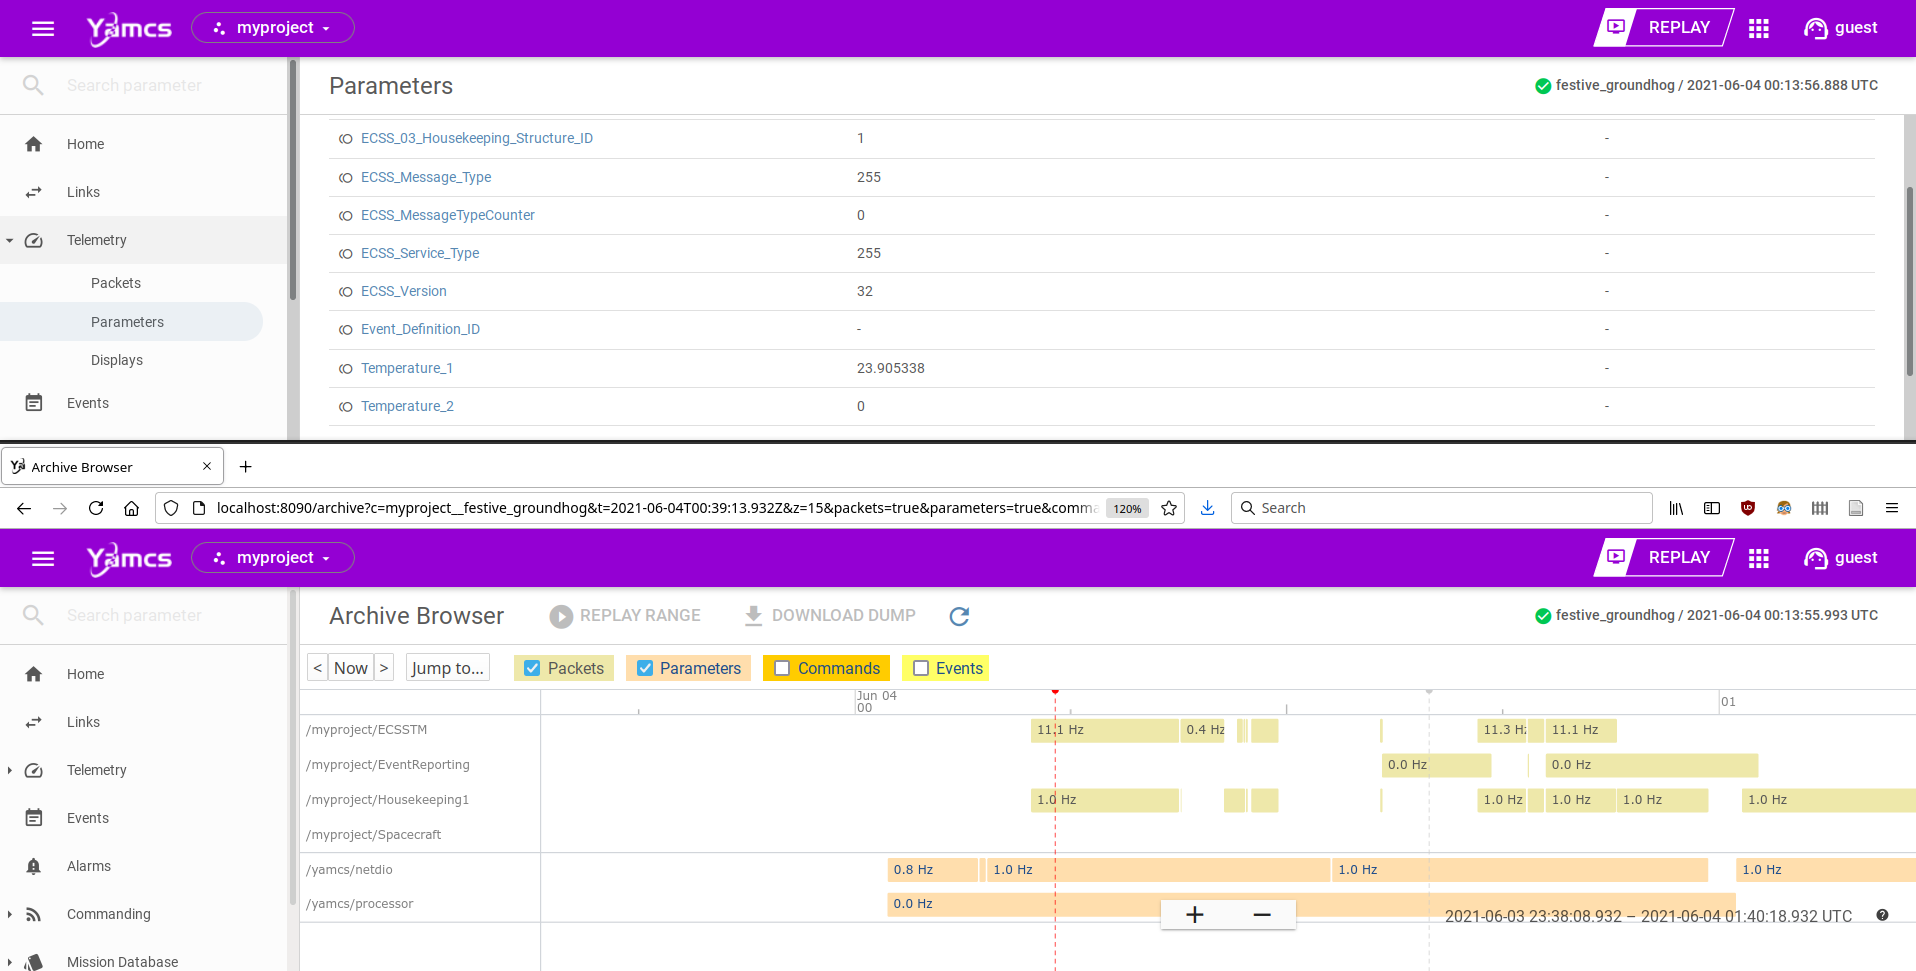
\includegraphics{screenshots/yamcs_replay}
	\caption{\acs{YAMCS} parameter and archive views}
\end{figure}

\section{\ac{FDIR} setup}

The purpose of the test setup is to observe the response of the system to any failure of the two "vulnerable" temperature sensors. For this purpose, we will attempt to simulate every failure mode of each sensor, and design an \ac{FDIR} implementation that anticipates all those failures.

\marginnote{Double failures are not investigated in the scope of this document, as they are mostly considered only for launchers and manned missions \parencite{SAVOIR-HB-003}.}
As a required input for the \ac{FDIR} detailed design, a \ac{FMEA} analysis needs to be prepared for the system. All \ac{FMEA} performed follows the requirements of the ECSS-Q-ST-30-02C standard.\autocite{ECSS-Q-ST-30-02C} The analysis is based on the \ac{FMEA} performed for the AcubeSAT nanosatellite,\autocite{retselis_acubesat_fmea_2020} and can be seen in \Cref{tab:fmea} for the reduced system. All expected failure modes for the two sensors are investigated, as well as a failure mode for the entire system that can be detected by correctly-operating sensors. Each of those failure modes will be later verified by injecting software or hardware modifications.

\begin{table*}[h]
	\centering
	\caption[][10pt]{\acs{FMEA} on demonstration system}
	\label{tab:fmea}
	\begin{adjustbox}{width=1.05\textwidth,center}
	\begin{tabular}{@{}lL{4cm}L{2cm}L{1cm}L{4cm}L{2cm}L{4cm}L{1.5cm}L{3cm}@{}}
		\toprule
		\multicolumn{1}{l}{ID}                            & Failure Mode                     & Failure Cause(s)     & Mission Phase     & Failure effects: Local                                    & Failure effects: End effects & Failure Detection/Observable symptoms                                               & Severity level & Compensating provisions             \\ \midrule
		\multicolumn{9}{l}{Temperature sensor MCP9808 \#1}                                                                                                                                                                                                                                                                                                                                                               \\ \midrule
		\textbf{\texttt{F-010}}                                      & Temporary loss of function       & Intrinsic, Radiation & All & No temperature measurement from this sensor               & None                         & No communication via \acs{I2C}                                                            & 4              & Dual-redundant temperature sensor   \\
		\textbf{\texttt{F-020}}                                      & Permanent loss of function       & Intrinsic, Radiation & All & No temperature measurement from this sensor               & None                         & No communication via \acs{I2C}                                                            & 4              & Dual-redundant temperature sensor   \\
		\textbf{\texttt{F-030}}                                      & Short Circuit between power pins & Intrinsic, Radiation & All & No temperature measurement from this sensor               & None                         & No communication via \acs{I2C}                                                            & 4              & Current-limiting resistor           \\
		\textbf{\texttt{F-040}}                                      & Temporary Value Shift            & Intrinsic, Radiation & All & Incorrect temperature readings                            & None                         & Temperature difference between 2 redundant sensors bigger than a safety value  & 4              & Dual-redundant temperature sensor   \\
		\textbf{\texttt{F-050}}                                      & Permanent Value Shift            & Intrinsic, Radiation & All & Incorrect temperature readings                            & None                         & Temperature difference between 2 redundant sensors bigger than a safety value  & 4              & Dual-redundant temperature sensor   \\
		\textbf{\texttt{F-060}}                                      & \acs{I2C} bus pin output stuck         & Intrinsic, Radiation & All & Inability to communicate with both sensors & None                         & No communication via \acs{I2C} for all temperature sensors                                & 4              & Sensors wired on separate \acs{I2C} buses \\
		\midrule
		\multicolumn{9}{l}{Temperature sensor MCP9808 \#2}                        \\ \midrule
		\textbf{\texttt{F-070}}                                      & Temporary loss of function       & Intrinsic, Radiation & All & No temperature measurement from this sensor               & None                         & No communication via \acs{I2C}                                                            & 4              & Dual-redundant temperature sensor   \\
		\textbf{\texttt{F-080}}                                      & Permanent loss of function       & Intrinsic, Radiation & All & No temperature measurement from this sensor               & None                         & No communication via \acs{I2C}                                                            & 4              & Dual-redundant temperature sensor   \\
		\textbf{\texttt{F-090}}                                      & Short Circuit between power pins & Intrinsic, Radiation & All & No temperature measurement from this sensor               & None                         & No communication via \acs{I2C}                                                            & 4              & Current-limiting resistor           \\
		\textbf{\texttt{F-100}}                                      & Temporary Value Shift            & Intrinsic, Radiation & All & Incorrect temperature readings                            & None                         & Temperature difference between 2 redundant sensors bigger than a safety value & 4              & Dual-redundant temperature sensor   \\
		\textbf{\texttt{F-110}}                                      & Permanent Value Shift            & Intrinsic, Radiation & All & Incorrect temperature readings                            & None                         & Temperature difference between 2 redundant sensors bigger than a safety value  & 4              & Dual-redundant temperature sensor   \\
		\textbf{\texttt{F-120}}                                      & \acs{I2C} bus pin output stuck         & Intrinsic, Radiation & All & Inability to communicate with both sensors & None                         & No communication via \acs{I2C} for all temperature sensors                                & 4              & Sensors wired on separate \acs{I2C} buses \\ \midrule
		\multicolumn{9}{l}{Subsystem}                        \\ \midrule
		\textbf{\texttt{F-130}}                                      & Overheating       & Short circuit, Environmental & All & Vulnerable component failure             & Loss of subsystem functionality           & Measured temperature outside expected range  & 3              & Thermal analysis with uncertainty margins, overcurrent protection   \\
		\bottomrule
	\end{tabular}
	\end{adjustbox}
\end{table*}

\subsection{\ac{FDIR} detailed design}

\begin{figure*}[ht]
	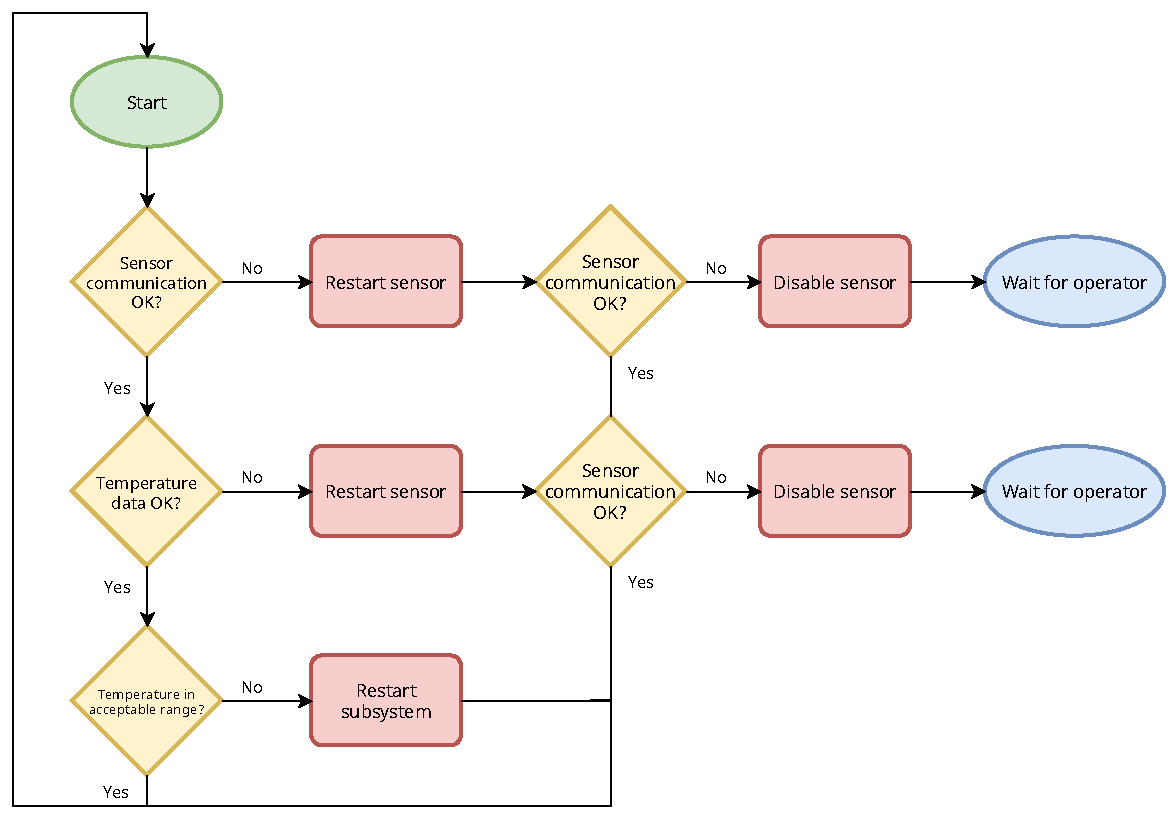
\includegraphics{TempSensorFDIR}
	\caption{Overview of the temperature sensor \ac{FDIR} process}
	\label{fig:fdirtemp}
\end{figure*}

The \ac{FDIR} of the sensors follows the hierarchical process described in \Cref{sec:fdir_operating_modes}, which is shown in \Cref{fig:fdirtemp} as tailored for the sensors.

The approach acts using the following steps, which are constantly being executed in the background:
\marginnote{For this demonstration, we will not investigate failures of the microcontroller itself and its internals. Refer to \parencite{retselis_acubesat_fmea_2020} for AcubeSAT's \acs{FMEA} and \acs{HSIA} on the microcontrollers.}
\begin{compactenum}
	\item The \ac{I2C} bus health status is monitored. Any failure or lack of communication indicates a failure in the sensor's electronics.
	\item The temperature output of the sensors is monitored. Any values which are outside the bounds of the physically possible thermal conditions are considered to indicate sensor or communication failures. Any values outside the operational limits of the subsystem's electronics are considered to indicate overheating and lead to a subsystem restart.
	\item In order to recover from the failures, first a restart of the sensor is attempted. If the erroneous values still persist, then the sensor cannot recover from the failure, but is just isolated and disabled instead.
\end{compactenum}

\clearpage
\paragraph{\acl{HSIA}}

After defining the possible failure modes and logic of the system, we are ready to analyse each entry to provide the correct software inputs to implement the required \ac{FDIR}. More specifically, for each failure, the following must be defined: \autocite[84]{SAVOIR-HB-003}
\begin{compactitem}
	\item Parameters to be monitored for detection
	\item Value ranges to be used to warn that a parameter is exceeding a specified range
	\item Isolation and reconfiguration actions to prevent failure propagation and, if possible, bring the system to a well operating state
\end{compactitem}

The above information is listed in the \acf{HSIA} table, which links each failure (identified in the \acl{FMEA}) to the corresponding low-level software parameters (\Cref{tab:hsia}).

For the purposes of this demonstration, we will consider that all \ac{FMEA} items can lead to \emph{feared events}, i.e. that \ac{FDIR} will anticipate all identified possible failures.

The \ac{HSIA} adds the following significant pieces of information to the \ac{FMEA}:\autocite{ECSS-Q-ST-30-02C}
\begin{itemize}
	\item The \textbf{monitored parameters} and the \textbf{conditions} that trigger the recovery action.
	
	These are listed here in terms of \ac{PUS} parameters which can be easily identified and compared by software. This list is then linked to the corresponding \emph{\texttt{ST[12]} on-board monitoring} service definitions, listed in \Cref{tab:demo_monitoring}.
	
	It is important to note that no single out-of-bounds value can trigger a recovery action. This is recommended in order to prevent transient errors or temporary communication protocol issues from triggering an unnecessary response which might disable a well-functioning component.
	
	\marginnote{\textbf{Temporary failure}: Caused by events such as bit flips, noise or transients, and can be corrected without intervention, or with a simple restart/power-cycle.\par\textbf{Permament failure}: A failure (typically in hardware, e.g. due to latchups or short-circuits) that cannot be corrected autonomously.}
	The distinction between \emph{temporary} and \emph{permanent} failures is made by \textbf{counting the number of consecutive failures}. Before a permanent action to disable a sensor is enacted, at least 5 attempts to communicate must have failed.
	
	The use of 2 hot-redundant sensor also allows us to investigate the difference between the two temperatures to deduce the health of the produced data. If the absolute difference between the 2 values is too high, assuming the sensors are placed close enough together, an error condition is assumed. However, as triple modular redundancy was not implemented for this system, it is not possible to deduce which sensor has failed.
	
	\item The \textbf{failure recovery and isolation actions}.
	
	These are listed in terms of \ac{PUS} events (\emph{\texttt{ST[05]} event reporting}) and event-actions (\emph{\texttt{ST[19]} eventaction}), which are linked to \Cref{tab:demo_eventaction}.
	
	The selected recovery actions match the approach shown in \Cref{fig:fdirtemp}. Additionally, when it is not known which sensor has failed, a fail-safe approach of restarting or disabling both sensors is used.
\end{itemize}

\begin{table*}
	\centering
	\caption{HSIA table}
	\label{tab:hsia}
	\begin{tabular}{@{}lL{4cm}L{4cm}L{1cm}L{1cm}L{3.5cm}@{}}
		\toprule
		ID & Failure Mode & Monitored Parameters & Monitoring ID & Event ID & Failure Recovery Action \\ \midrule
		\multicolumn{6}{l}{Temperature sensor MCP9808 \#1} \\ \midrule
		
		
		
		\textbf{\texttt{F-010}} & Temporary loss of function & \(\texttt{T1\_Status} = \texttt{TIMEOUT}\) \newline for 2 times & 0 & 0 & Power-cycle sensor 1 \\
		\textbf{\texttt{F-020}} & Permanent loss of function & \(\texttt{T1\_Status} = \texttt{TIMEOUT}\) \newline for 5 times & 2 & 2 & Ignore sensor 1 values \\
		\textbf{\texttt{F-030}} & Short Circuit between power pins & \(\texttt{T1\_Status} = \texttt{TIMEOUT}\) \newline for 5 times & 2 & 2 & Ignore sensor 1 values \\[5ex]
		\textbf{\texttt{F-040}} & Temporary Value Shift & 
		\(
		\begin{cases}
			\left|\Delta T\right| & > \SI{20}{\celsius} \text{ or} \\
			T_1 &> \SI{100}{\celsius} \text{ or} \\
			T_1 &< \SI{-40}{\celsius}
		\end{cases}
		\) \newline for 2 times
		 & 4, 6 & 0, 4 & Power-cycle sensor 1 \\
		\textbf{\texttt{F-050}} & Permanent Value Shift & \(
		\begin{cases}
		\left|\Delta T\right| & > \SI{20}{\celsius} \text{ or} \\
		T_1 &> \SI{100}{\celsius} \text{ or} \\
		T_1 &< \SI{-40}{\celsius}
		\end{cases}
		\) \newline for 5 times & 7, 9 & 2, 5 & Ignore sensor 1 values \\[9ex]
		\textbf{\texttt{F-060}} & \acs{I2C} bus pin output stuck & \(\texttt{T1\_Status} = \texttt{TIMEOUT}\) \newline for 5 times & 2 & 2 & Ignore sensor 1 values \\ \midrule
		
		
		
		\multicolumn{6}{l}{Temperature sensor MCP9808 \#2} \\ \midrule
		
		
		
		\textbf{\texttt{F-070}} & Temporary loss of function & \(\texttt{T2\_Status} = \texttt{TIMEOUT}\) \newline for 2 times & 1 & 1 & Power-cycle sensor 2 \\
		\textbf{\texttt{F-080}} & Permanent loss of function & \(\texttt{T2\_Status} = \texttt{TIMEOUT}\) \newline for 5 times & 3 & 3 & Ignore sensor 2 values \\
		\textbf{\texttt{F-090}} & Short Circuit between power pins & \(\texttt{T2\_Status} = \texttt{TIMEOUT}\) \newline for 5 times & 3 & 3 & Ignore sensor 2 values \\[5ex]
		\textbf{\texttt{F-100}} & Temporary Value Shift & 
		\(
		\begin{cases}
		\left|\Delta T\right| & > \SI{20}{\celsius} \text{ or} \\
		T_2 &> \SI{100}{\celsius} \text{ or} \\
		T_2 &< \SI{-40}{\celsius}
		\end{cases}
		\) \newline for 2 times
		& 5, 6 & 1, 4 & Power-cycle sensor 2 \\
		\textbf{\texttt{F-110}} & Permanent Value Shift & \(
		\begin{cases}
		\left|\Delta T\right| & > \SI{20}{\celsius} \text{ or} \\
		T_2 &> \SI{100}{\celsius} \text{ or} \\
		T_2 &< \SI{-40}{\celsius}
		\end{cases}
		\) \newline for 5 times & 8, 9 & 3, 5 & Ignore sensor 2 values \\[9ex]
		\textbf{\texttt{F-120}} & \acs{I2C} bus pin output stuck & \(\texttt{T2\_Status} = \texttt{TIMEOUT}\) \newline for 5 times & 3 & 3 & Ignore sensor 2 values \\ \midrule
		
		
		
		\multicolumn{6}{l}{Subsystem} \\ \midrule
		
		
		
		\textbf{\texttt{F-130}} & Overheating & \(T_1 > \SI{40}{\celsius}\) or \(T_2 > \SI{40}{\celsius}\) & 10, 11 & 6 & Restart subsystem \\ \bottomrule
	\end{tabular}
	\vspace{2pt}
\end{table*}

\clearpage

\paragraph{Parameters}

After investigating the \acl{HSIA}, we can list the scalar parameters for the \emph{\texttt{ST[20]} parameter management} service\autocite{ECSS-E-ST-70-41C} (\Cref{tab:demo_params}).

Beyond the actual temperature values, we have included the \textbf{difference} (\(\Delta\)) between the two temperatures, since the \acs{PUS} standard does not provide ways to perform arithmetic calculations without hard-coded software. Additionally, the status of each sensor peripheral is included, which is an enumerated value.\footnote{One of \texttt{NOMINAL}, \texttt{TIMEOUT} or \texttt{DISABLED}} 

These parameters are telemetered to the ground segment and displayed to the user periodically, via the \emph{\texttt{ST[03]} housekeeping} \ac{PUS} service. However, during flight, the ground segment will not have constant access, since the satellite will not be visible from ground stations throughout its entire orbit.

\begin{table}[h]
	\centering
	\caption[List of \texttt{ST[20]} parameters]{List of \texttt{ST[20]} parameters\\R: Read-only\\RW: Read-write}
	\label{tab:demo_params}
	\begin{tabularx}{\textwidth}{@{}rlllX@{}}
		\toprule
		Param. ID & Parameter              & Units & Type & Type \\ \midrule
		0            & Temperature 1          & \si{\celsius}      & \texttt{float} & R     \\
		1            & Temperature 2          & \si{\celsius}      & \texttt{float} & R    \\
		2            & \(\Delta\) Temperature & \si{\celsius}      & \texttt{float} & R    \\
		3            & Temperature 1 Status         &       & Enumerated   & RW  \\
		4            & Temperature 2 Status         &       & Enumerated   & RW  \\
		5			 & Temperature 1+2 Status       &		& Enumerated   & R  \\ \bottomrule
	\end{tabularx}
\end{table}

\paragraph{On-board monitoring definitions}

After defining the parameters, the monitoring definitions that establish the acceptable and actionable ranges for each parameter should be outlined. These are then managed by the \emph{\texttt{ST[12]} on-board monitoring} \ac{PUS} service.

The \emph{check validity conditions} are important to mention in this case, as they use the three \emph{Status} parameters to prevent executing checks for disabled peripherals. As such, sensors that are not providing values due to hardware issues, \ac{FDIR} actions or operator intervention, will not be able to trigger \ac{FDIR} actions.

\begin{table*}[h]
	\centering
	\caption[List of \texttt{ST[12]} monitoring definitions][5pt]{List of \texttt{ST[12]} monitoring definitions. \(t\) and \(\Delta\) are used as placeholders for parameter values.}
	\label{tab:demo_monitoring}
	\begin{adjustbox}{width=\textwidth}
	\begin{tabular}{@{}L{1cm}L{2.5cm}L{2.8cm}L{2cm}L{2cm}L{2cm}ll@{}}
		\toprule
		&  & \multicolumn{2}{c}{Check validity condition} &  &  & \multicolumn{2}{c}{Check} \\ \cmidrule(lr){3-4} \cmidrule(l){7-8} 
		Definition ID & Monitored Parameter & Validity Parameter & Expected Value & Monitoring Interval & Repetition Number & Check Type & Criteria \\ \midrule
		0 & Temp. 1 Status &  &  & \SI{500}{\milli\second} & 2 & Expected Value & \(\neq\) \texttt{TIMEOUT} \\
		1 & Temp. 2 Status &  &  & \SI{500}{\milli\second} & 2 & Expected Value & \(\neq\) \texttt{TIMEOUT} \\
		2 & Temp. 1 Status &  &  & \SI{500}{\milli\second} & 5 & Expected Value & \(\neq\) \texttt{TIMEOUT} \\
		3 & Temp. 2 Status &  &  & \SI{500}{\milli\second} & 5 & Expected Value & \(\neq\) \texttt{TIMEOUT} \\
		\midrule
		4 & Temperature 1 & Temp. 1 Status & \texttt{NOMINAL} & \SI{500}{\milli\second} & 2 & Range & \( -\SI{40}{\celsius} < t < \SI{100}{\celsius} \) \\
		5 & Temperature 2 & Temp. 2 Status & \texttt{NOMINAL} & \SI{500}{\milli\second} & 2 & Range & \( -\SI{40}{\celsius} < t < \SI{100}{\celsius} \) \\
		6 & \(\Delta\) Temperature & Temp. 1+2 Status & \texttt{NOMINAL} & \SI{500}{\milli\second} & 2 & Range & \( -\SI{20}{\celsius} < \Delta < \SI{20}{\celsius} \) \\
		\midrule
		7 & Temperature 1 & Temp. 1 Status & \texttt{NOMINAL} & \SI{500}{\milli\second} & 5 & Range & \( -\SI{40}{\celsius} < t < \SI{100}{\celsius} \) \\
		8 & Temperature 2 & Temp. 2 Status & \texttt{NOMINAL} & \SI{500}{\milli\second} & 5 & Range & \( -\SI{40}{\celsius} < t < \SI{100}{\celsius} \) \\
		9 & \(\Delta\) Temperature & Temp. 1+2 Status & \texttt{NOMINAL} & \SI{500}{\milli\second} & 5 & Range & \( -\SI{20}{\celsius} < \Delta < \SI{20}{\celsius} \) \\
		\midrule
		10 & Temperature 1 & Temp. 1 Status & \texttt{NOMINAL} & \SI{500}{\milli\second} & 5 & Range & \( t < \SI{50}{\celsius} \) \\
		11 & Temperature 2 & Temp. 2 Status & \texttt{NOMINAL} & \SI{500}{\milli\second} & 5 & Range & \( t < \SI{50}{\celsius} \) \\ \bottomrule
	\end{tabular}
	\end{adjustbox}
\end{table*}

\paragraph{Event-action definitions}

The final part of the puzzle are the event-action definitions, which can be seen on \Cref{tab:demo_eventaction} and combine:
\begin{itemize}
	\item \ac{PUS} events (\texttt{ST[05]} service) which are automatically generated when an on-board monitoring definition goes out of limits
	\item \ac{PUS} event-action definitions (\texttt{ST[19]} service), which link every occurrence of an event to a stored \ac{TC} that is immediately executed.
	They define the \acs{FDIR} recovery actions.
\end{itemize}

All the aforementioned definitions can be easily modified by operators using single commands that affect the on-board stored \ac{PUS} database.

\begin{table}[h]
	\centering
	\caption{List of \texttt{ST[19]} event-action definitions}
	\label{tab:demo_eventaction}
	\begin{tabular}{@{}lL{2cm}L{7cm}@{}}
		\toprule
		Event ID & Monitoring Definitions & Action \\ \midrule
		0 & 0, 4 & Restart sensor 1 \\
		1 & 1, 5 & Restart sensor 2 \\
		2 & 2, 7 & Set sensor 1 status \( = \) \texttt{DISABLED} \\
		3 & 3, 8 & Set sensor 2 status \( = \) \texttt{DISABLED} \\
		4 & 6 & Restart all sensors \\
		5 & 9 & Set all sensors status \( = \) \texttt{DISABLED} \\
		6 & 10, 11 & Restart system \\ \bottomrule
	\end{tabular}
\end{table}

\clearpage
\section{\ac{FDIR} validation}

\subsection{Nominal operation}

During nominal operation, no failures are simulated. The system is connected to power and outputs \ac{ECSS} telemetry (\Cref{fig:yamcshousekeeping}), which includes parameter values parsed by (\Cref{fig:yamcsparameter}). Additionally, a log file is kept for diagnostic purposes (\Cref{fig:lognominal}). The system is compliant with its requirements (\Cref{sec:tsvcd}) and can transmit the temperature to the ground station as expected.

\begin{figure}
	\centering
	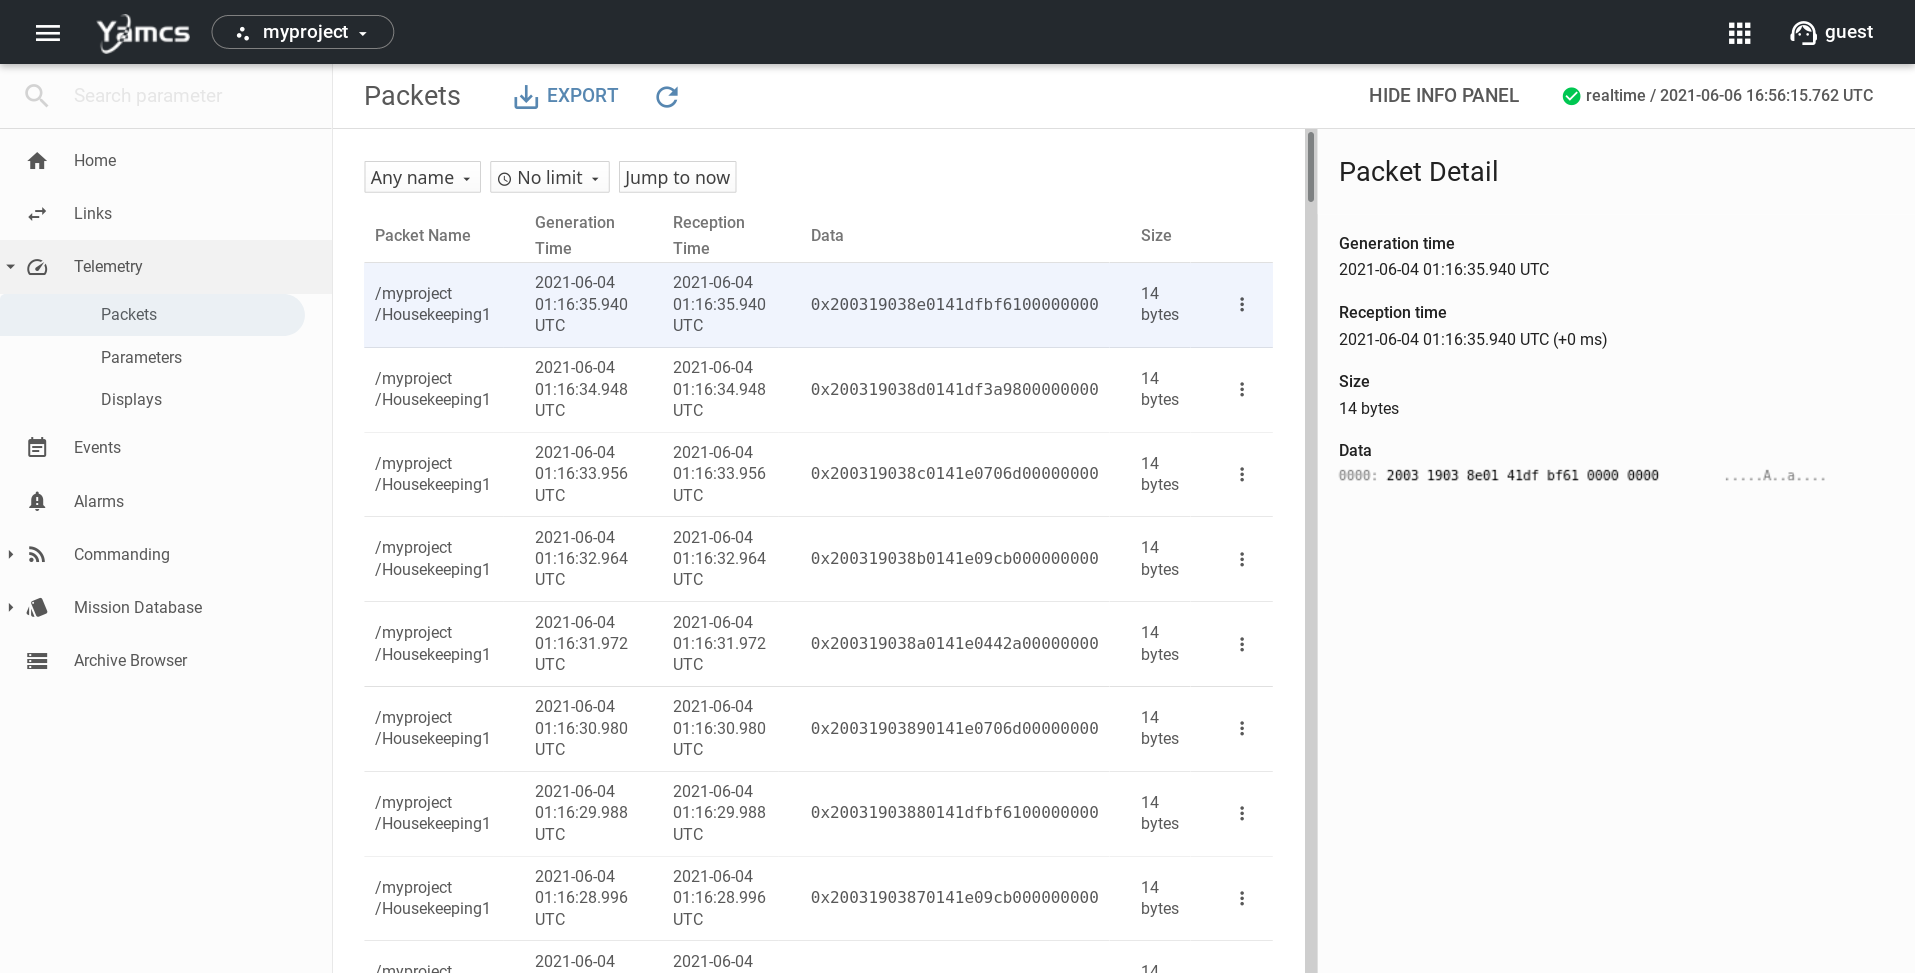
\includegraphics{media/screenshots/yamcs_housekeeping}
	\caption{View of housekeeping packets generated by the \acs{MCU} in \acs{YAMCS}}
	\label{fig:yamcshousekeeping}
\end{figure}

\begin{figure}[h]
	\centering
	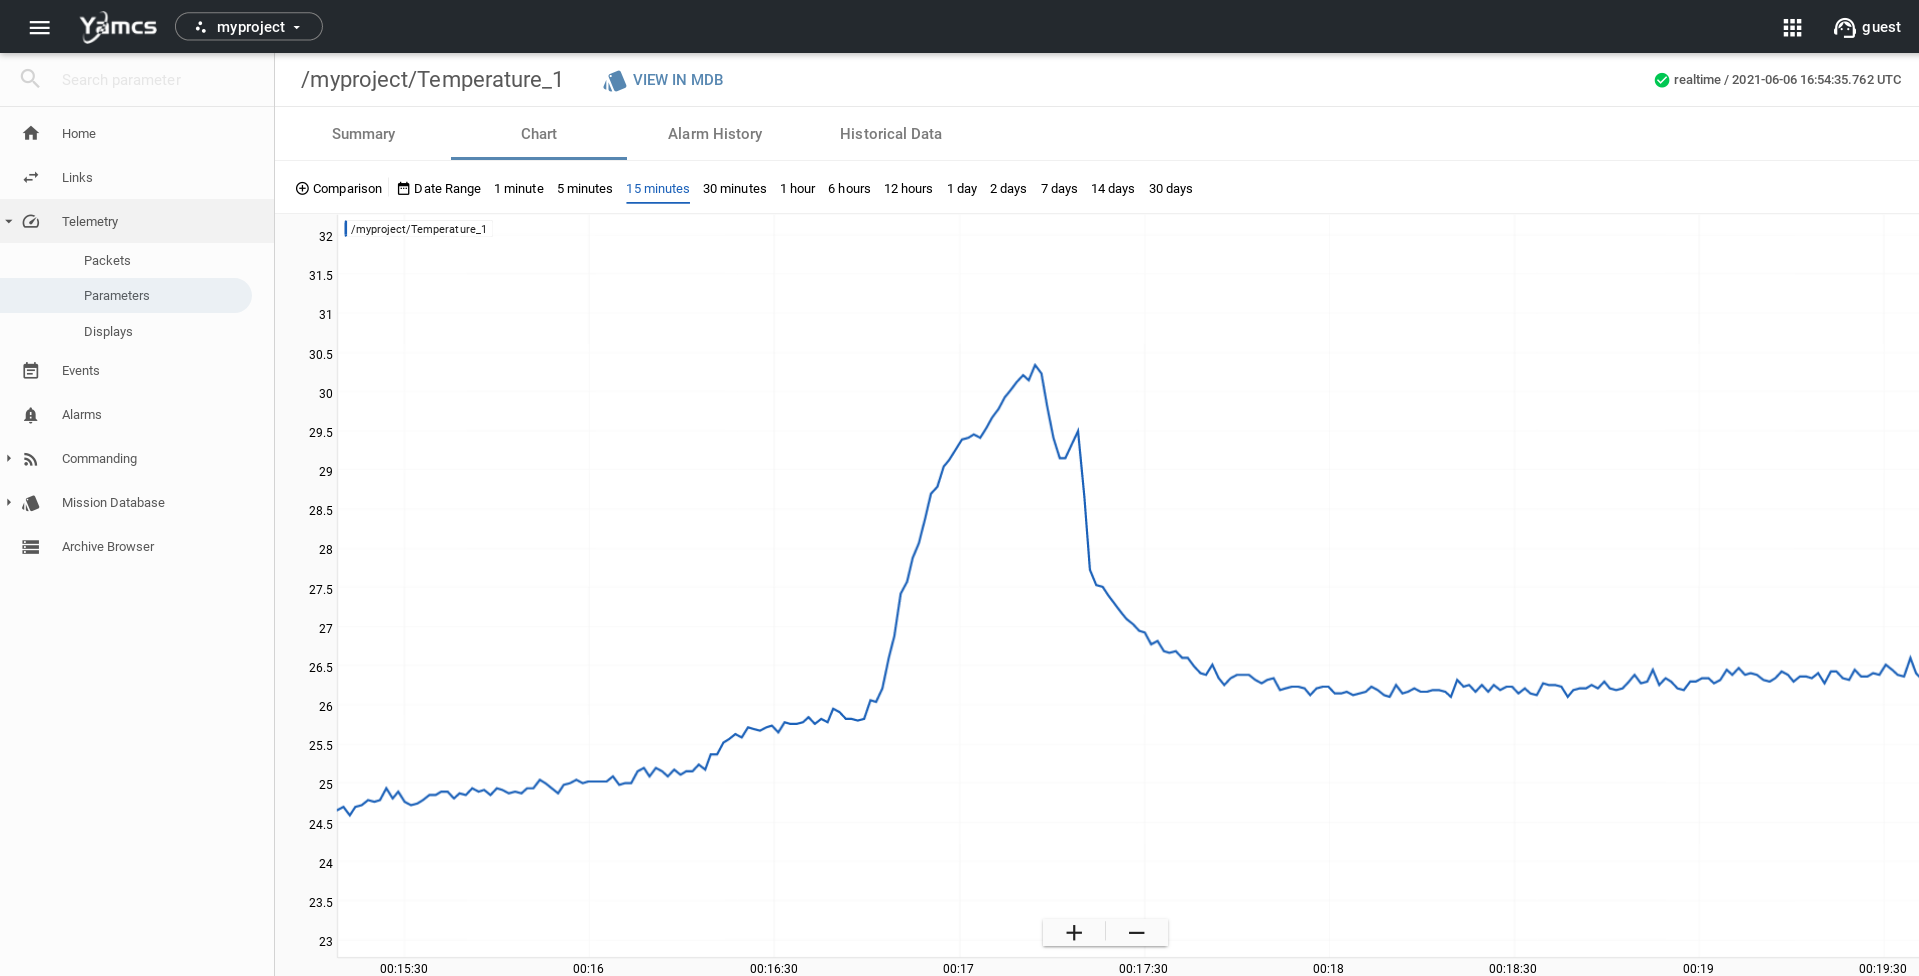
\includegraphics{media/screenshots/yamcs_parameter}
	\caption{View of one temperature parameter in \acs{YAMCS}}
	\label{fig:yamcsparameter}
\end{figure}

\begin{figure}
\begin{cminted}{text}
909601  [debug  ] T1 = 28.18
909701  [debug  ] T1 = 28.08
909801  [debug  ] T1 = 28.14
909901  [debug  ] T1 = 27.97
910000  [trace  ] New TM [3,25]
910001  [debug  ] T1 = 28.10
910101  [debug  ] T1 = 28.03
910201  [debug  ] T1 = 28.12
910301  [debug  ] T1 = 27.90
910401  [debug  ] T1 = 28.08
\end{cminted}
\caption[Log output during nominal operation]{Log output during nominal operation. The first number is the \ac{MCU} tick counter in milliseconds since boot.}
\label{fig:lognominal}
\end{figure}

\subsection{Simulation of failures}

The following methods were used to simulate each failure:
\begin{itemize}
	\item For component communication failures, each sensor was just physically disconnected from the system.
	\item For small changes in temperature, a hot air gun or other hot air source was pointed towards each sensor. Care was taken to not exceed the rated temperatures of the affected components.
	\item For changes in temperature which were impractical to simulate, the failure was injected in software, by manually modifying the variable.
	
	The two buttons present on the development board were used as a simple interface to "inject" extreme temperature values.
\end{itemize}

\subsection{Real-time modification of \ac{FDIR}}

The power of \acs{SAVOIR}'s \ac{FDIR} approach lies in the fact that the entire \ac{FDIR} concept can be safely modified via \ac{TC} without requiring any modifications or reuploads of the spacecraft's software. The application of the \acs{ECSS} services paradigm allows customising all on-board \ac{FDIR} functions and associated services using predefined \ac{TC} structures. In this section, \acs{ECSS} commands will be executed to demonstrate these capabilities and their control from the Ground Station.

The level of reconfigurability possible is defined by requirements listed in \parencite{ECSS-E-ST-70-11C,SAVOIR-HB-003}. The tailored version used for our experiments is listed in \Cref{tab:fdir-recon-rq}.

\begin{table*}[h]
	\centering
	\caption{\ac{FDIR} reconfigurability requirements}
	\label{tab:fdir-recon-rq}
	\begin{tabularx}{\textwidth}{@{}lXlL{4cm}@{}}
		\toprule
 		\# & Requirement & Service & Details \\ \midrule
		\texttt{RC-010} & The reporting of FDIR activities shall contain all information for failure analysis (e.g. time of occurrence, parameter out‐of‐limit, switching performed). & ST[12] on-board monitoring & Via periodic \emph{check transition reports} \\
		\texttt{RC-020} & The capability shall be provided to enable and to disable any on‐board FDIR function by telecommand. & ST[12] on-board monitoring & Via \emph{enable}/\emph{disable} \emph{parameter monitoring definitions} commands  \\
		\texttt{RC-030} & The capability shall be provided to add and delete parameters from the on‐board monitoring list. & ST[12] on-board monitoring & Via \emph{add}/\emph{delete} \emph{parameter monitoring definitions} commands  \\
		\texttt{RC-040} & The capability shall be provided to modify the failure recovery actions associated with each on-board monitoring definition. & ST[19] event-action & Via \emph{add}, \emph{delete}, \emph{enable} and \emph{disable} \emph{event-action definitions} commands \\ \bottomrule
	\end{tabularx}
\end{table*}

The \ac{YAMCS} platform was once again used to generate the wanted commands (\Cref{fig:yamcs_commands}).

\begin{figure}[h]
	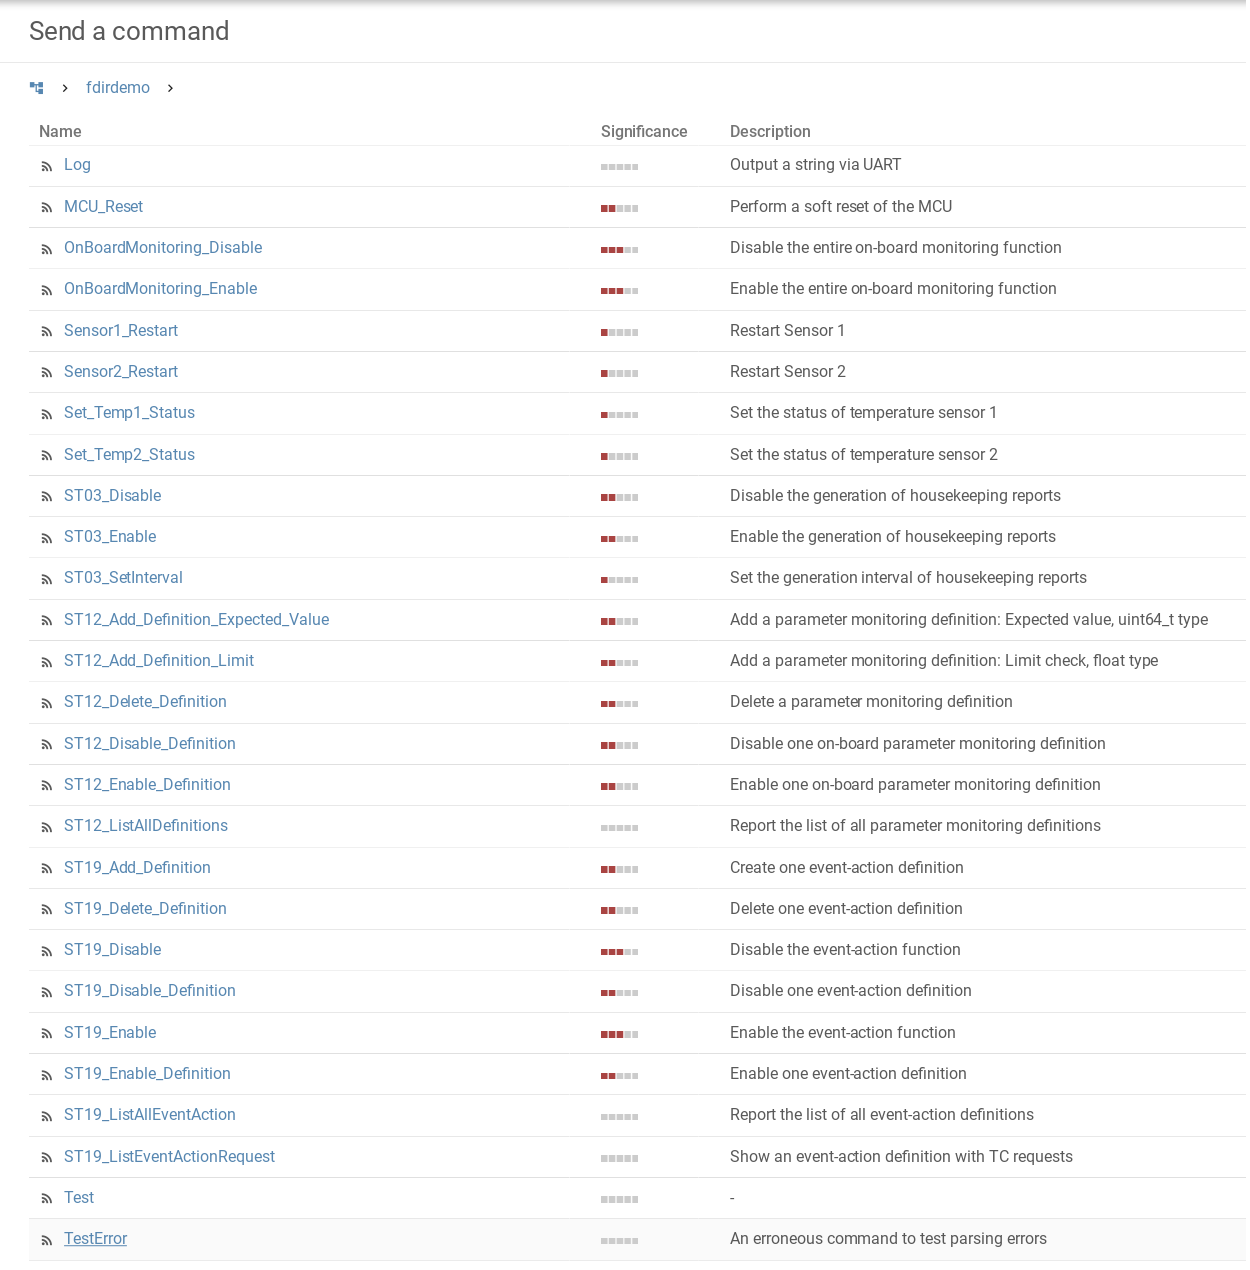
\includegraphics{screenshots/yamcs_commands.png}
	\caption{List of commands in the \acs{YAMCS} interface. These commands can initiate spacecraft actions, enable/disable sensors, or reconfigure the on-board \acs{ECSS} services databases. The list of commands is provided programmatically in \ac{XTCE} format (\Cref{app:xtce}).}
	\label{fig:yamcs_commands}
\end{figure}





\chapter{Conclusions and Future Work}

% Suggestions for standard:
% hard to play with parameters
% two validity conditions: safe mode etc. how to manage?
% derived parameters (e.g. Δ between sensors)
% event-action definition ID

\section{Future work}

%\backmatter
\appendix

\begin{fullwidth}
\printbibliography[heading=bibnumbered]
\end{fullwidth}


\printindex

\chapter{Source code}
\label{sec:source_code}

\setminted{
	bgcolor={},
	fontsize=\fontsize{9pt}{9pt}
}

%\begin{fullwidth}

\section*{\texttt{main.cpp}}

%\inputminted{cpp}{code/main.cpp}

\newpage
\section*{\texttt{xtce.xml}}
\label{app:xtce}

fixme

%\inputminted{xml}{code/xtce.xml}

%\end{fullwidth}

\end{document}

